\documentclass[12pt,a4paper]{report}

\usepackage[T1]{fontenc}
\usepackage[utf8]{inputenc}
\usepackage{times}
\usepackage{setspace}
\usepackage{geometry}
\usepackage{titlesec}
\usepackage{graphicx}
\usepackage{float}
\usepackage{longtable}
\usepackage{booktabs}
\usepackage{array}
\usepackage{enumitem}
\usepackage[hidelinks]{hyperref}
\usepackage{amsmath}
\usepackage{amssymb}
\usepackage{tikz}
\usepackage{pgfplots}
\usepackage{caption}
\usepackage{fancyhdr}
\usepackage{url}
\usepackage[table]{xcolor}
\usepackage{listings}
\usepackage{microtype}
\usepackage{xurl}

\pgfplotsset{compat=1.18}
\usetikzlibrary{arrows.meta, positioning, shapes.geometric, shapes.misc, calc, fit, matrix, shadows.blur}

% Allow long strings / URLs to break in tables and paragraphs
\emergencystretch=2em

% KUET format
\geometry{
  top=1.2in,
  bottom=1.0in,
  left=1.2in,
  right=1.0in,
  headsep=0.2in,
  footskip=0.4in
}

\onehalfspacing
\renewcommand{\bibname}{References}

\titleformat{\chapter}[display]
  {\bfseries\centering\fontsize{16}{18}\selectfont}
  {CHAPTER \thechapter}
  {0.5em}
  {}

\titleformat{\section}
  {\bfseries\fontsize{14}{16}\selectfont}
  {\thesection}
  {0.7em}
  {}

\titleformat{\subsection}
  {\bfseries\fontsize{12}{14}\selectfont}
  {\thesubsection}
  {0.7em}
  {}

\captionsetup[figure]{font={normalsize},justification=centering}
\captionsetup[table]{font={normalsize},justification=centering}

\definecolor{kuetblue}{RGB}{0,71,171}
\definecolor{kuetgray}{RGB}{245,247,250}

\newcommand{\screenshotplaceholder}[1]{%
  \begin{figure}[H]
    \centering
    \fbox{\parbox[c][2.0in][c]{0.85\textwidth}{\centering Screenshot Placeholder\\[4pt] #1}}
    \caption{#1}
  \end{figure}
}

\newcommand{\realshot}[3]{%
  \begin{figure}[H]
    \centering
    \includegraphics[width=#1\textwidth]{#2}
    \caption{#3}
  \end{figure}
}

\begin{document}

\hypersetup{pageanchor=false}

% Front matter: two unnumbered title pages (cover + inner), then roman from Acknowledgment
\pagenumbering{roman}
\setcounter{page}{1}
% Two title pages (cover + inner). Tighter vertical spacing; \singlespacing avoids
% global \onehalfspacing from stretching these pages.

\newcommand{\TitleCoverBlock}{%
\begingroup
\fontsize{18}{27}\selectfont\bfseries\scshape
A PROJECT REPORT\par
\vspace{3pt}
ON\par
\vspace{5pt}
COGNITIVE COPILOT: AI-POWERED ACADEMIC LEARNING\par
\vspace{3pt}
MANAGEMENT SYSTEM WITH LOCAL LLM INTEGRATION\par
\endgroup}

\newcommand{\DeptFooterBlock}{%
\begingroup
\fontsize{12}{14.4}\selectfont\bfseries
Department of Computer Science and Engineering\par
Khulna University of Engineering \& Technology\par
Khulna 9203, Bangladesh\par
\vspace{0.25\baselineskip}
\normalfont April 2026\par
\endgroup}

\begin{titlepage}
\thispagestyle{empty}
\begingroup
\singlespacing
\vspace*{18pt}
\begin{center}
{\fontsize{14}{16}\selectfont\normalfont CSE 3200: System Development Project\par}

\vspace{12pt}

\TitleCoverBlock

\vspace{14pt}

{\fontsize{14}{16}\selectfont\normalfont By\par}

\vspace{16pt}

{\fontsize{14}{16}\selectfont\bfseries Khadimul Islam Mahi\par}
\vspace{1pt}
{\fontsize{14}{16}\selectfont\normalfont Roll: 2107076\par}

\vspace{0.38in}

{\fontsize{14}{16}\selectfont\bfseries \&\par}

\vspace{0.14in}

{\fontsize{14}{16}\selectfont\bfseries Sumaiya Akter\par}
\vspace{1pt}
{\fontsize{14}{16}\selectfont\normalfont Roll: 2107080\par}

\vspace{8pt}


\includegraphics[width=1.14in,height=1.0in,keepaspectratio]{figures/Logo_KUET.svg.png}

\vspace{14pt}

\DeptFooterBlock
\end{center}
\endgroup
\end{titlepage}

\newcommand{\TitleInnerBlock}{%
\begingroup
\fontsize{18}{27}\selectfont\bfseries\normalfont
Cognitive Copilot: AI-Powered Academic Learning\par
\vspace{4pt}
Management System with Local LLM Integration\par
\endgroup}

\begin{titlepage}
\thispagestyle{empty}
\begingroup
\singlespacing
\vspace*{20pt}
\begin{center}
\TitleInnerBlock

\vspace{16pt}

{\fontsize{12}{18}\selectfont\normalfont By\par}

\vspace{12pt}

{\fontsize{12}{18}\selectfont\bfseries Khadimul Islam Mahi\par}
\vspace{1pt}
{\fontsize{12}{18}\selectfont\normalfont Roll: 2107076\par}

\vspace{0.12in}

{\fontsize{12}{18}\selectfont\bfseries \&\par}

\vspace{0.12in}

{\fontsize{12}{18}\selectfont\bfseries Sumaiya Akter\par}
\vspace{1pt}
{\fontsize{12}{18}\selectfont\normalfont Roll: 2107080\par}
\end{center}

\vspace{20pt}

\noindent{\fontsize{12}{18}\selectfont\bfseries Supervisor:\par}
\vspace{3pt}
\noindent\hspace*{0.8in}%
\begin{minipage}[t]{\dimexpr\textwidth-0.8in\relax}
{\fontsize{12}{18}\selectfont\bfseries Md. Nazirul Hasan Shawon\par}
\vspace{2pt}
{\fontsize{12}{18}\selectfont\bfseries Lecturer\par}
{\fontsize{12}{18}\selectfont\normalfont Department of Computer Science and Engineering\par
Khulna University of Engineering \& Technology\par}
\vspace{8pt}
\noindent\rule{2.35in}{0.45pt}\par
\vspace{2pt}
{\fontsize{12}{18}\selectfont\normalfont Signature}\par
\end{minipage}

\vspace{14pt}

\begin{center}
{\fontsize{11}{13.2}\selectfont\normalfont
\textbf{CSE 3200: System Development Project}\par}
\vspace{8pt}
\DeptFooterBlock
\end{center}
\endgroup
\end{titlepage}

\setcounter{page}{1}
\chapter*{Acknowledgment}
\addcontentsline{toc}{chapter}{Acknowledgment}

We would like to express our sincere gratitude to our supervisor, Md. Nazirul Hasan Shawon, Professor, Department of Computer Science and Engineering, KUET, for his guidance, valuable feedback, and constant encouragement during the completion of this project.

We are also thankful to the faculty members and lab staff of the Department of CSE, KUET, for providing the academic environment and technical facilities required to carry out this work.

Finally, we would like to thank our families and friends for their support and motivation throughout the project period.

\vspace{1cm}
\noindent
Khadimul Islam Mahi (Roll: 2107076)\\
Sumaiya Akter (Roll: 2107080)

\clearpage
\chapter*{Abstract}
\addcontentsline{toc}{chapter}{Abstract}

This report presents \textbf{Cognitive Copilot}, a full-stack academic learning platform that combines core Learning Management System (LMS) workflows with an AI tutor. The project is built around practical university needs: course and topic management, classroom community interactions, routine and attendance support, notifications, and AI-assisted study. The system is implemented as a web application with a React frontend and a FastAPI backend.

The implementation follows a modular architecture. The frontend provides role-based pages for students and tutors, while the backend exposes REST APIs for authentication, courses, routine, community, analytics, settings, profile, materials, and notifications. For AI functionality, the platform integrates local model inference with retrieval-based question answering and quiz support in the AI Tutor workspace. OCR-assisted ingestion and asynchronous workers support long-running operations so user interactions stay responsive.

The project emphasizes engineering reliability over experimental claims. The report therefore focuses on implemented modules, data flow, CRUD behaviors, validation and authorization design, and tested user workflows. No unsupported performance or accuracy numbers are presented as final evidence; instead, verification is described through reproducible build and test procedures across backend and frontend.

Cognitive Copilot demonstrates how a project can remain academically meaningful while also being implementation-driven: it delivers a unified learning environment, keeps AI features integrated with course context, and preserves maintainable software structure suitable for further extension in future academic work.

\clearpage

\tableofcontents
\clearpage
\listoftables
\clearpage
\listoffigures
\clearpage

% Main matter
\hypersetup{pageanchor=true}
\pagenumbering{arabic}
\setcounter{page}{1}

\chapter{Introduction}

\section{Introduction}
A single tool is seldom enough for academic life today. Students balance course portals, separate channels for help, and improvised AI assistants that do not know which subject or reading they should follow. That everyday friction is what led us to build \textbf{Cognitive Copilot}: a web application where routine LMS work and AI-assisted study share the same accounts, the same course data, and the same expectations about roles and permissions.

This chapter states the background and the problem we set out to solve, together with the objectives and scope, why the idea is not a direct copy of any single existing product, how we planned the work, and how we divided responsibilities between team members.

\section{Background and Problem Statement}
Academic workflows in many universities are still spread across several tools. Students often use one system for courses, another for communication, and separate platforms for AI support. That fragmentation means constant context switching and weak continuity between teaching materials and study support.

\textbf{Cognitive Copilot} is built as one platform that combines LMS workflows and AI qssisted study. It is not meant to replace classroom teaching, but to offer a structured digital space where students and tutors interact around the same course information.

The following practical problems motivated us:
\begin{enumerate}[label=\arabic*.]
\item Course resources, routine, and communication are not unified in a single workflow.
\item AI chat tools are often detached from course materials, which leads to low context answers.
\item Many systems offer partial features, but CRUD behavior, validation, and role based interactions are not always handled consistently.
\item When the architecture is not modular, deployment and maintenance become difficult.
\end{enumerate}

\section{Objectives}
This work has the following aims:
\begin{enumerate}[label=\arabic*.]
\item Implement a role aware LMS with core modules: authentication, courses, routine, community, notifications, analytics, settings, and profile.
\item Build an AI Tutor workspace merged with course and topic context and several study modes.
\item Support practical material workflows such as upload and retrieval assisted question answering.
\item Keep CRUD operations reliable across modules with clear request validation and authorization checks.
\item Deliver a deployable full stack implementation suitable for local development and demonstration.
\end{enumerate}

\section{Scope of the Project (Modern Tools and Boundaries)}
The implemented scope includes:
\begin{itemize}
\item User authentication, profile, and settings management.
\item Course, topic, and material management.
\item Routine and attendance related workflows.
\item Community classrooms, threads, announcements, and member interactions.
\item A notification feed with real time update handling.
\item Analytics dashboards for students and tutors.
\item AI Tutor modes for guided learning interactions.
\end{itemize}

Out of scope items for this report include native mobile clients and institution-wide multi-tenant deployment policies.

The frontend is built with React, TypeScript, and Vite; TanStack Query and Zustand help with server state and UI state. The backend uses Python with FastAPI and Pydantic, and SQLAlchemy for asynchronous access to PostgreSQL. Redis supports caching and background jobs; workers handle longer tasks such as ingestion and OCR. Docker Compose containerizes the stack for a reproducible local environment. These choices reflect what is sustainable for a student project while still aligning with common industry practice.

\section{Unfamiliarity of the Problem, Topic, and Solution}
Neither an LMS nor an AI tutor is new by itself. What we set out to do differently is \emph{integration under one engineering story}: the same role model, the same course entities, and the same API discipline for both traditional LMS pages and the AI Tutor workspace. We did not mirror a single commercial product; we composed open patterns (REST APIs, modular services, retrieval assisted answering, local model hosting) into a system that fits our course requirements.

Our contribution is best described as \textbf{software integration and dependable behavior}---clear contracts between modules, validated inputs, and tutor flows that stay tied to course and topic context---rather than claiming a new learning algorithm. Chapter~II discusses related work and situates this project among existing systems and research directions.

\section{Project Planning and Work Distribution}
We organized the work in overlapping phases: requirements and module boundaries, backend foundations (auth, schema, core CRUD), frontend pages aligned with those APIs, the AI Tutor and asynchronous ingestion, then integration, testing, and report writing. Where possible we used short iterations: implement a slice end to end, stabilize it, then move on.

Both team members worked across frontend and backend; we split ownership mainly by module to limit conflicting edits and to keep reviews focused. One member led authentication, profile, settings, routine, and analytics-related paths; the other led courses and materials, community, notifications, and the AI Tutor UI and wiring. Shared tasks included database modeling decisions, Docker-based integration testing, diagram preparation, and final proofreading of the report. A formal Gantt chart is not included as a figure in this version, but the chapter order of the report follows the sequence we used in development.

\section{Report Organization}
The remainder of the report is organized as follows:
\begin{itemize}
\item Chapter~II describes applications of the work, how the repository is organized, related literature, and a short discussion of novelty.
\item Chapter~III presents methodology: analysis, architecture, and modeling diagrams.
\item Chapter~IV covers experimental setup, evaluation, implementation, results, and how objectives were met.
\item Chapter~V addresses societal, ethical, legal, safety, and environmental considerations.
\item Chapter~VI maps the project to complex engineering problems and activities.
\item Chapter~VII concludes with summary, limitations, and future work.
\end{itemize}

\chapter{Related Works}

\section{Learning Management Platforms}
Traditional LMS services are centered around managing courses, assignment management, and grading. Their operational strength is strong.
but AI-assisted learning is external or less connected. This forms a general disjunction: students are able to.
access information, yet contextual tutoring is not combined with the same course data.

\section{AI-Assisted Learning Systems}
Recent AI tutoring systems demonstrate the importance of interactive question answering, guided explanation, and adaptive practice.
Nonetheless, most of the implementations rely on generic chat interactions with little grounding in course. In educational settings,
examples are more effective when associated with real class content and subject matter.

|human|>section Retrieval-Augmented Generation in Education.
Retrieval-Augmented Generation (RAG) is a combination of language generation with information retrieval. This is in course contexts.
helpful since answers can be linked to existing resources, rather than model memory alone. Current research
promotes hybrid retrieval strategies integrating lexical and vector cues \cite{lewis2020rag,gao2023ragsurvey).
	
	In this project, the corresponding notion is not an originality in designing algorithms, but a practical application of retrieval to.
	Answers to course context in LMS.
	
	OCR in Academic Processes.
	Digitization of documents has been a long term use of OCR. Old-fashioned OCR engines are effective in clean printed text, whereas.
	OCR with methods based on transformers is under investigation in more complicated cases. OCR can be of use in the educational processes.
	to extract text on uploaded content or timetable image to allow content to be indexed and re-used.
section Agentic and Multi-Mode Tutor Interfaces.
In many instances, a modern tutor interface will be a combination of more than one interaction pattern: free chat, explain mode, question answering, quiz.
resource recommendations, practice and. The associated body of literature on tool-using agents and structured prompting.
This direction is informed by cite: react-yao2023 and toolformer-schick2023. In this case, the focus of this report is on implemented.
instead of hypothetical agent performance assertions.

section. Location of this Project.
According to the context above, Cognitive Copilot is a positioned implementation-based academic system that:
\begin{itemize}
	item combines LMS modules and AI tutor processes into a single platform,
	item connects AI interactions to course/topic context,
	item assists with real-world classroom activities (community, notifications, routine, analytics),
	item and emphasizes correctness and maintainability of software.
\end{itemize}

Engineering integration and interoperability of modules is the project contribution but not a claim of a.
new AI algorithm.
\chapter{Methodology}
\label{ch:design}

\section{Introduction}
This chapter explains \emph{how} we approached the system: the constraints we respected, the layered architecture we chose, and the modeling artifacts (use case, structural, behavioral, deployment, and data-flow views) that make the implementation easier to reason about. The focus stays on methodology and design rationale; detailed run configuration and test evidence appear in Chapter~IV.

\section{Problem Design and Analysis}
\subsection{Design principles}
The project has the following design principles:
\begin{enumerate}[label=\arabic*.]
	\item \textbf{Modularity:} frontend is clearly separated from API, services and data layers.
	\item \textbf{Know your user:} separate actions for students and tutors handled in the UI and API.
	\item \textbf{Reliability first:} background tasks are used to ensure responsiveness.
	\item \textbf{Maintainability:} API contracts and schema validation are used.
\end{enumerate}

\subsection{Core functional actors}
The system supports three role patterns:
\begin{itemize}
\item \textbf{Student:} learns through courses, AI Tutor, routine, and community.
\item \textbf{Tutor:} manages class operations, announcements, and monitoring views.
\item \textbf{Admin-level control:} extends management and moderation operations where configured.
\end{itemize}

\section{Overall Framework and System Architecture}
The deployed architecture has four main layers:
\begin{itemize}
\item \textbf{Frontend:} React + TypeScript application for all user-facing pages.
\item \textbf{Backend API:} FastAPI service handling authentication, CRUD, and business logic.
\item \textbf{Data and Queue Layer:} PostgreSQL for persistence and Redis for cache/queue support.
\item \textbf{AI and Worker Layer:} local model integration and worker processes for long-running jobs.
\end{itemize}

\begin{figure}[htbp]
\centering
\resizebox{0.92\textwidth}{!}{%
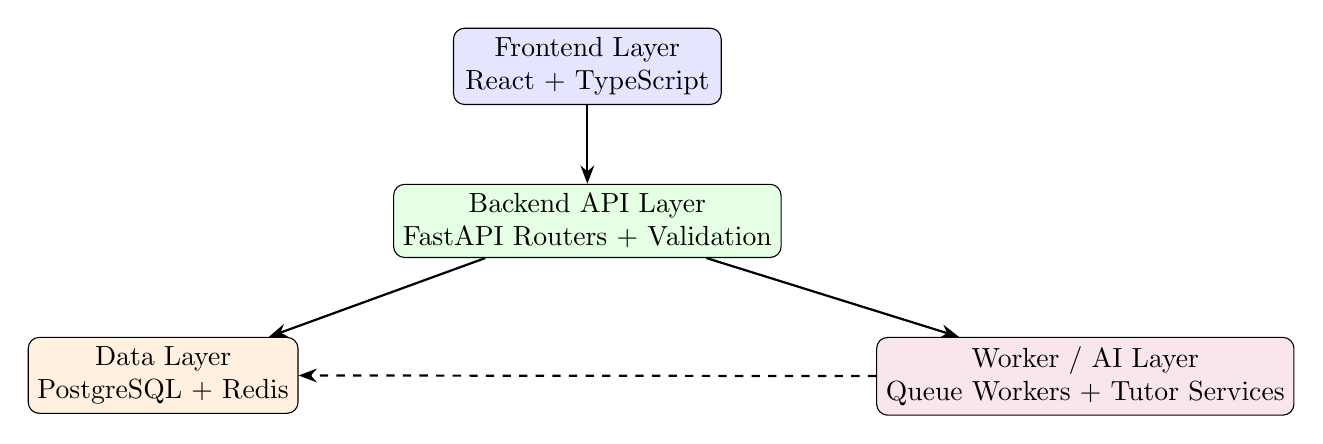
\begin{tikzpicture}[
    node distance=10mm and 12mm,
    layer/.style={draw, rounded corners, align=center, minimum width=3.4cm, minimum height=9mm, fill=kuetgray},
    arr/.style={-{Stealth}, thick}
]
\node[layer, fill=blue!10] (frontend) {Frontend Layer\\React + TypeScript};
\node[layer, fill=green!10, below=of frontend] (api) {Backend API Layer\\FastAPI Routers + Validation};
\node[layer, fill=orange!12, below left=of api] (data) {Data Layer\\PostgreSQL + Redis};
\node[layer, fill=purple!10, below right=of api] (worker) {Worker / AI Layer\\Queue Workers + Tutor Services};

\draw[arr] (frontend) -- (api);
\draw[arr] (api) -- (data);
\draw[arr] (api) -- (worker);
\draw[arr, dashed] (worker) -- (data);
\end{tikzpicture}
}
\caption{Layered architecture of the Cognitive Copilot system.}
\label{fig:system-layer-arch}
\end{figure}

\section{Use Case Diagram}
\begin{figure}[htbp]
\centering
\resizebox{0.90\textwidth}{!}{%
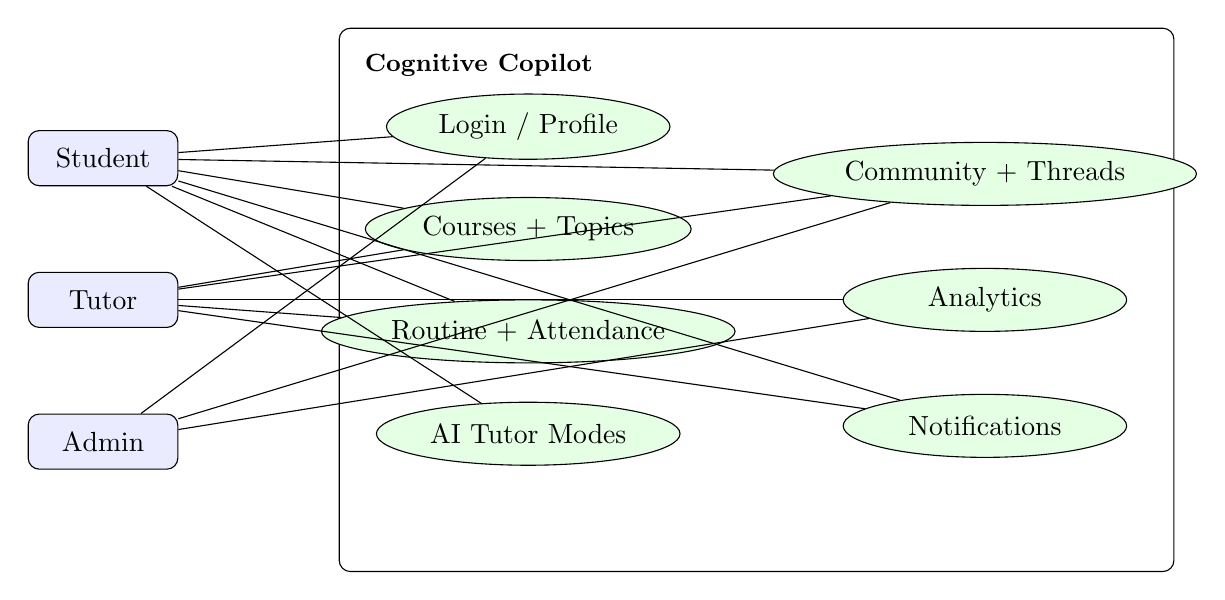
\begin{tikzpicture}[
    actor/.style={draw, rounded corners, align=center, minimum width=1.9cm, minimum height=7mm, fill=blue!8},
    usecase/.style={ellipse, draw, align=center, minimum width=3.6cm, minimum height=8mm, fill=green!10},
    boundary/.style={draw, rounded corners, minimum width=10.6cm, minimum height=6.9cm},
    link/.style={-}
]
\node[boundary] (sys) at (1.7,0) {};
\node[anchor=north west, font=\small\bfseries] at (-3.4,3.25) {Cognitive Copilot};

\node[actor] (student) at (-6.6,1.8) {Student};
\node[actor] (tutor) at (-6.6,0.0) {Tutor};
\node[actor] (admin) at (-6.6,-1.8) {Admin};

\node[usecase] (auth) at (-1.2,2.2) {Login / Profile};
\node[usecase] (courses) at (-1.2,0.9) {Courses + Topics};
\node[usecase] (routine) at (-1.2,-0.4) {Routine + Attendance};
\node[usecase] (aitutor) at (-1.2,-1.7) {AI Tutor Modes};
\node[usecase] (community) at (4.6,1.6) {Community + Threads};
\node[usecase] (analytics) at (4.6,0.0) {Analytics};
\node[usecase] (notify) at (4.6,-1.6) {Notifications};

\draw[link] (student) -- (auth);
\draw[link] (student) -- (courses);
\draw[link] (student) -- (routine);
\draw[link] (student) -- (aitutor);
\draw[link] (student) -- (community);
\draw[link] (student) -- (notify);

\draw[link] (tutor) -- (courses);
\draw[link] (tutor) -- (routine);
\draw[link] (tutor) -- (community);
\draw[link] (tutor) -- (analytics);
\draw[link] (tutor) -- (notify);

\draw[link] (admin) -- (auth);
\draw[link] (admin) -- (community);
\draw[link] (admin) -- (analytics);
\end{tikzpicture}
}
\caption{Use case diagram of key actors and system interactions.}
\label{fig:use-case-diagram}
\end{figure}

\section{Core Data Domains}
The project data model is organized into practical domains:
\begin{itemize}
\item Identity and profile data
\item Course, enrollment, topic, and material data
\item Routine and attendance data
\item Community and thread interaction data
\item Notification and analytics data
\item AI tutor interaction and progress-related data
\end{itemize}

\section{Class Diagram (High Level)}
\begin{figure}[htbp]
\centering
\resizebox{0.95\textwidth}{!}{%
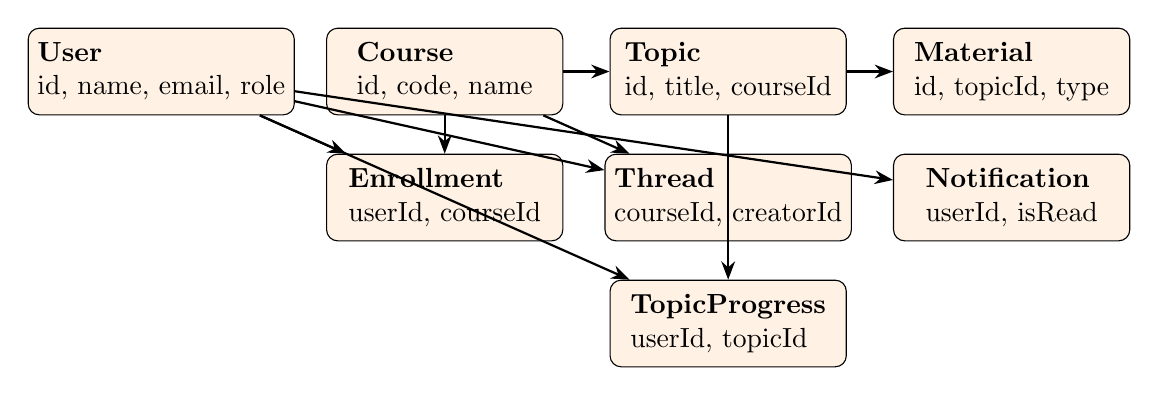
\begin{tikzpicture}[
    clsbox/.style={draw, rounded corners, align=left, minimum width=3.0cm, minimum height=1.1cm, fill=orange!10},
    rel/.style={-{Stealth}, thick}
]
\node[clsbox] (user) at (-4.6,1.9) {\textbf{User}\\id, name, email, role};
\node[clsbox] (course) at (-1.0,1.9) {\textbf{Course}\\id, code, name};
\node[clsbox] (topic) at (2.6,1.9) {\textbf{Topic}\\id, title, courseId};
\node[clsbox] (material) at (6.2,1.9) {\textbf{Material}\\id, topicId, type};
\node[clsbox] (enroll) at (-1.0,0.3) {\textbf{Enrollment}\\userId, courseId};
\node[clsbox] (thread) at (2.6,0.3) {\textbf{Thread}\\courseId, creatorId};
\node[clsbox] (notification) at (6.2,0.3) {\textbf{Notification}\\userId, isRead};
\node[clsbox] (progress) at (2.6,-1.3) {\textbf{TopicProgress}\\userId, topicId};

\draw[rel] (user) -- (enroll);
\draw[rel] (course) -- (enroll);
\draw[rel] (course) -- (topic);
\draw[rel] (topic) -- (material);
\draw[rel] (user) -- (thread);
\draw[rel] (course) -- (thread);
\draw[rel] (user) -- (notification);
\draw[rel] (user) -- (progress);
\draw[rel] (topic) -- (progress);
\end{tikzpicture}
}
\caption{High level class relationship diagram for core entities.}
\label{fig:class-diagram}
\end{figure}

\section{ER Diagram (Conceptual)}
\begin{figure}[htbp]
\centering
\resizebox{0.86\textwidth}{!}{%
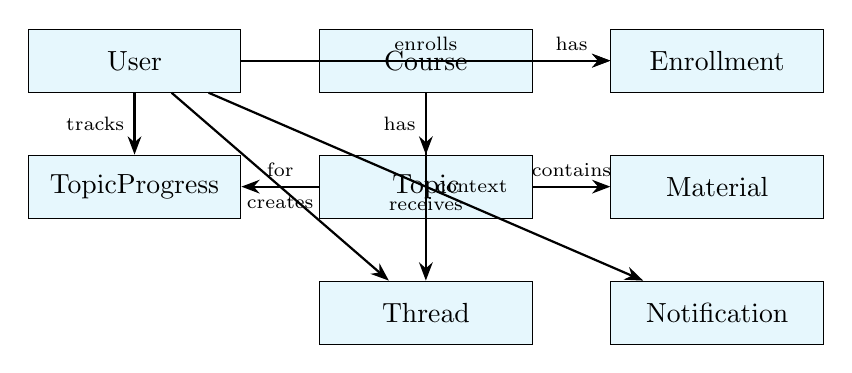
\begin{tikzpicture}[
    ent/.style={draw, rectangle, align=center, minimum width=2.7cm, minimum height=8mm, fill=cyan!10},
    rel/.style={-{Stealth}, thick}
]
\node[ent] (u)  at (-5.2, 2.2) {User};
\node[ent] (c)  at (-1.5, 2.2) {Course};
\node[ent] (e)  at ( 2.2, 2.2) {Enrollment};
\node[ent] (t)  at (-1.5, 0.6) {Topic};
\node[ent] (m)  at ( 2.2, 0.6) {Material};
\node[ent] (tp) at (-5.2, 0.6) {TopicProgress};
\node[ent] (th) at (-1.5,-1.0) {Thread};
\node[ent] (nt) at ( 2.2,-1.0) {Notification};

\draw[rel] (u) -- node[above, font=\scriptsize]{enrolls} (e);
\draw[rel] (c) -- node[above, font=\scriptsize]{has} (e);
\draw[rel] (c) -- node[left,  font=\scriptsize]{has} (t);
\draw[rel] (t) -- node[above, font=\scriptsize]{contains} (m);
\draw[rel] (u) -- node[left,  font=\scriptsize]{tracks} (tp);
\draw[rel] (t) -- node[above, font=\scriptsize]{for} (tp);
\draw[rel] (u) -- node[below, font=\scriptsize]{creates} (th);
\draw[rel] (c) -- node[right, font=\scriptsize]{context} (th);
\draw[rel] (u) -- node[below, font=\scriptsize]{receives} (nt);
\end{tikzpicture}
}
\caption{Conceptual ER diagram of the main project core tables.}
\label{fig:er-diagram}
\end{figure}
\section{Module Interaction Flow}
At run time the project has a uniform flow:
\begin{enumerate}[label=\arabic*.]
	\item API requests are made from the frontend pages.
	\item API validates data against schemas.
	\item Services enforce business rules and authentication.
	\item Data layer saves and returns normalized data.
	\item Frontend is kept in-sync with query cache and real-time updates.
\end{enumerate}

\begin{figure}[htbp]
\centering
\resizebox{0.96\textwidth}{!}{%
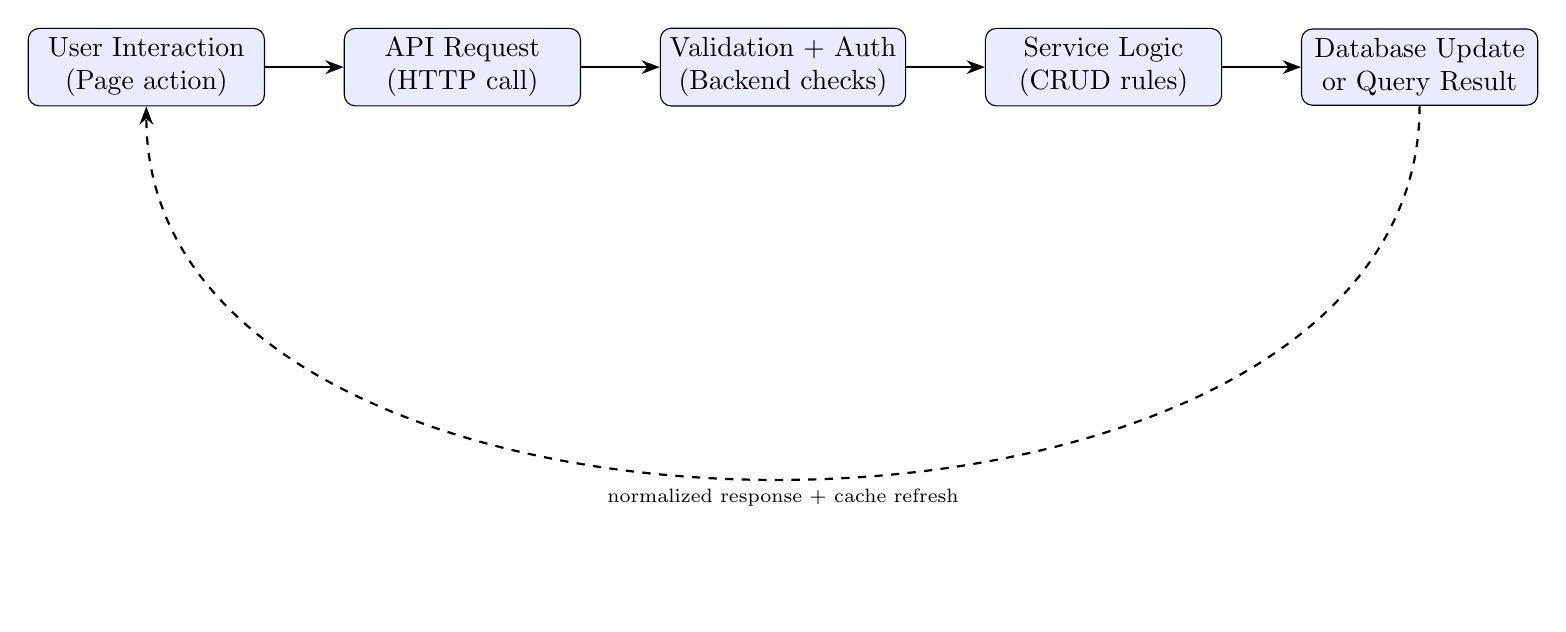
\begin{tikzpicture}[
    node distance=8mm and 10mm,
    flowstep/.style={draw, rounded corners, align=center, minimum width=3.0cm, minimum height=8mm, fill=blue!8},
    arr/.style={-{Stealth}, thick}
]
\node[flowstep] (s1) {User Interaction\\(Page action)};
\node[flowstep, right=of s1] (s2) {API Request\\(HTTP call)};
\node[flowstep, right=of s2] (s3) {Validation + Auth\\(Backend checks)};
\node[flowstep, right=of s3] (s4) {Service Logic\\(CRUD rules)};
\node[flowstep, right=of s4] (s5) {Database Update\\or Query Result};

\draw[arr] (s1) -- (s2);
\draw[arr] (s2) -- (s3);
\draw[arr] (s3) -- (s4);
\draw[arr] (s4) -- (s5);
\draw[arr, dashed] (s5.south) to[out=-90, in=-90] node[below, font=\scriptsize] {normalized response + cache refresh} (s1.south);
\end{tikzpicture}
}
\caption{End to end interaction flow from user action to synchronized UI state.}
\label{fig:module-flow}
\end{figure}

\section{Activity Diagram (Authentication Flow)}
\begin{figure}[htbp]
\centering
\resizebox{0.82\textwidth}{!}{%
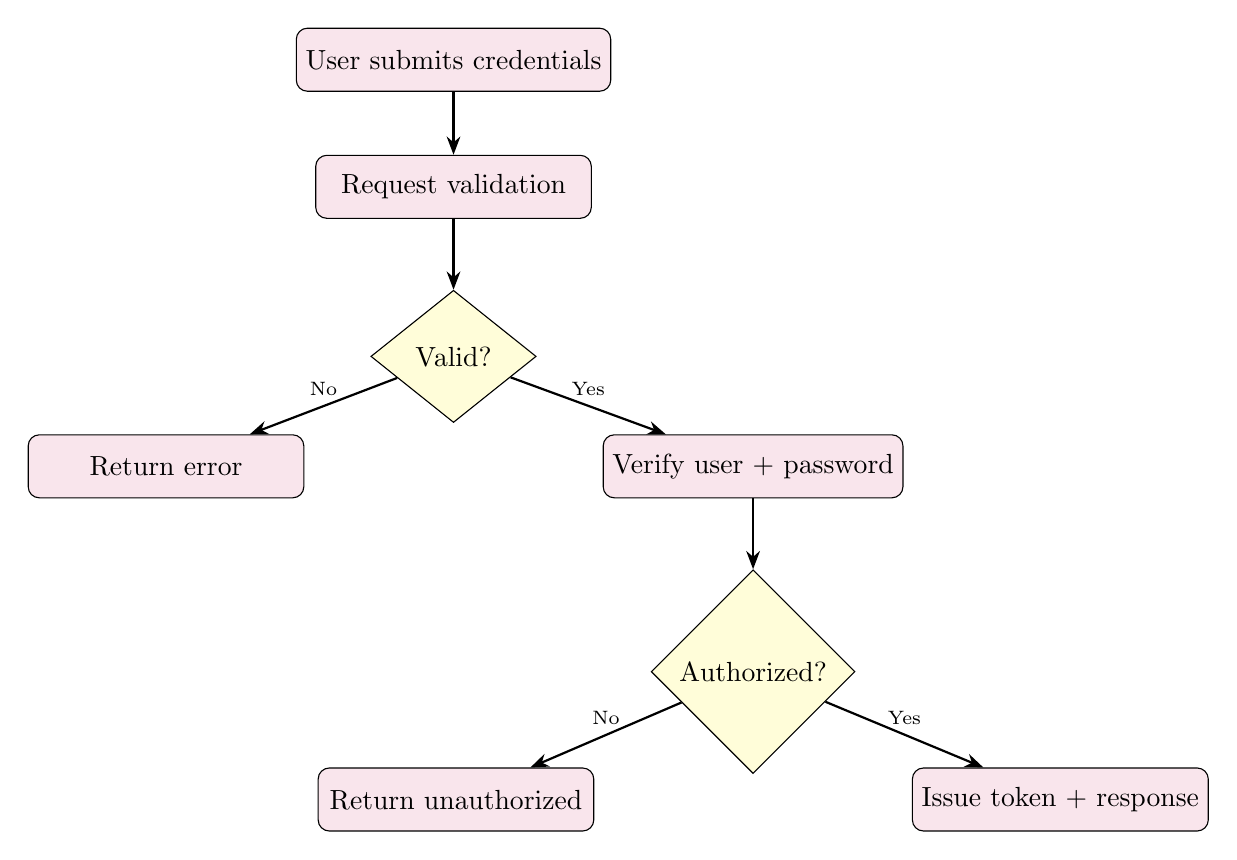
\begin{tikzpicture}[
    node distance=8mm,
    activity/.style={draw, rounded corners, align=center, minimum width=3.5cm, minimum height=8mm, fill=purple!10},
    decision/.style={diamond, draw, align=center, minimum width=2.1cm, minimum height=8mm, fill=yellow!15},
    arr/.style={-{Stealth}, thick}
]
\node[activity] (a1) {User submits credentials};
\node[activity, below=of a1] (a2) {Request validation};
\node[decision, below=of a2, yshift=-1mm] (d1) {Valid?};
\node[activity, below left=of d1, xshift=-8mm] (a3) {Return error};
\node[activity, below right=of d1, xshift=8mm] (a4) {Verify user + password};
\node[decision, below=of a4, yshift=-1mm] (d2) {Authorized?};
\node[activity, below left=of d2, xshift=-8mm] (a5) {Return unauthorized};
\node[activity, below right=of d2, xshift=8mm] (a6) {Issue token + response};

\draw[arr] (a1) -- (a2);
\draw[arr] (a2) -- (d1);
\draw[arr] (d1) -- node[above, font=\scriptsize]{No} (a3);
\draw[arr] (d1) -- node[above, font=\scriptsize]{Yes} (a4);
\draw[arr] (a4) -- (d2);
\draw[arr] (d2) -- node[above, font=\scriptsize]{No} (a5);
\draw[arr] (d2) -- node[above, font=\scriptsize]{Yes} (a6);
\end{tikzpicture}
}
\caption{Activity diagram for the authentication request lifecycle.}
\label{fig:activity-auth}
\end{figure}

\section{AI Tutor Methodology}
The AI Tutor is integrated as a module of the LMS rather than a separate chatbot. It supports multiple learning modes
through a shared workspace and course/topic context. Retrieval based answering and quiz workflows are connected with
existing course entities so interactions remain academically relevant.

\section{Sequence Diagram (AI Tutor Request)}
\begin{figure}[htbp]
\centering
\resizebox{0.92\textwidth}{!}{%
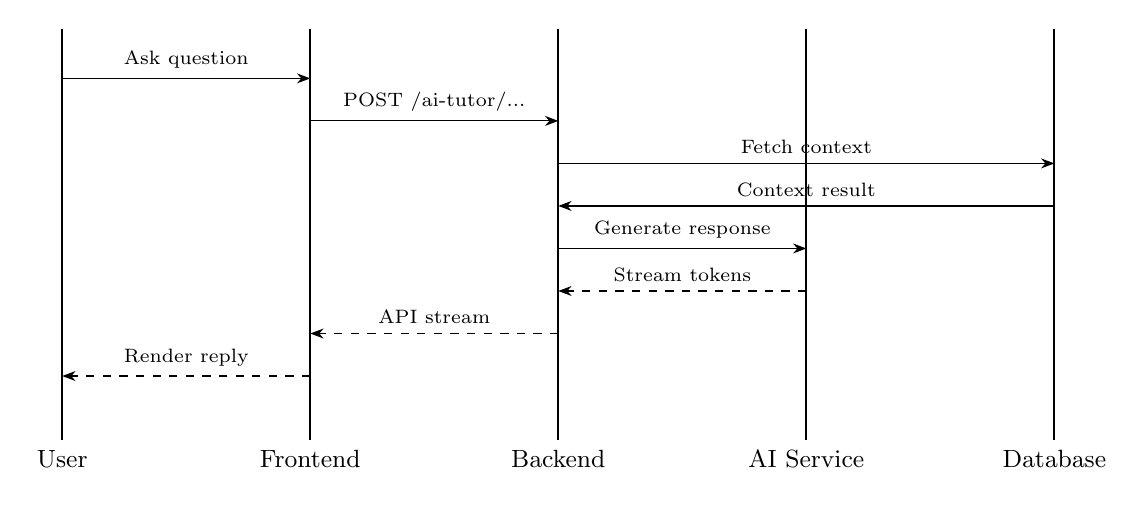
\begin{tikzpicture}[x=1.05cm,y=0.9cm, font=\small]
\draw[thick] (0,0) -- (0,-5.8) node[below] {User};
\draw[thick] (3,0) -- (3,-5.8) node[below] {Frontend};
\draw[thick] (6,0) -- (6,-5.8) node[below] {Backend};
\draw[thick] (9,0) -- (9,-5.8) node[below] {AI Service};
\draw[thick] (12,0) -- (12,-5.8) node[below] {Database};

\draw[-{Stealth}] (0,-0.7) -- (3,-0.7) node[midway,above,font=\scriptsize] {Ask question};
\draw[-{Stealth}] (3,-1.3) -- (6,-1.3) node[midway,above,font=\scriptsize] {POST /ai-tutor/...};
\draw[-{Stealth}] (6,-1.9) -- (12,-1.9) node[midway,above,font=\scriptsize] {Fetch context};
\draw[-{Stealth}] (12,-2.5) -- (6,-2.5) node[midway,above,font=\scriptsize] {Context result};
\draw[-{Stealth}] (6,-3.1) -- (9,-3.1) node[midway,above,font=\scriptsize] {Generate response};
\draw[-{Stealth}, dashed] (9,-3.7) -- (6,-3.7) node[midway,above,font=\scriptsize] {Stream tokens};
\draw[-{Stealth}, dashed] (6,-4.3) -- (3,-4.3) node[midway,above,font=\scriptsize] {API stream};
\draw[-{Stealth}, dashed] (3,-4.9) -- (0,-4.9) node[midway,above,font=\scriptsize] {Render reply};
\end{tikzpicture}
}
\caption{Sequence diagram for AI Tutor request and response flow.}
\label{fig:sequence-ai-tutor}
\end{figure}

\section{Asynchronous Processing Methodology}
For tasks that can be expensive (e.g., material ingestion and OCR), asynchronous worker execution is used. This prevents
HTTP request blocking, improves responsiveness, and allows safer retry and failure handling patterns.

\begin{figure}[htbp]
\centering
\resizebox{0.88\textwidth}{!}{%
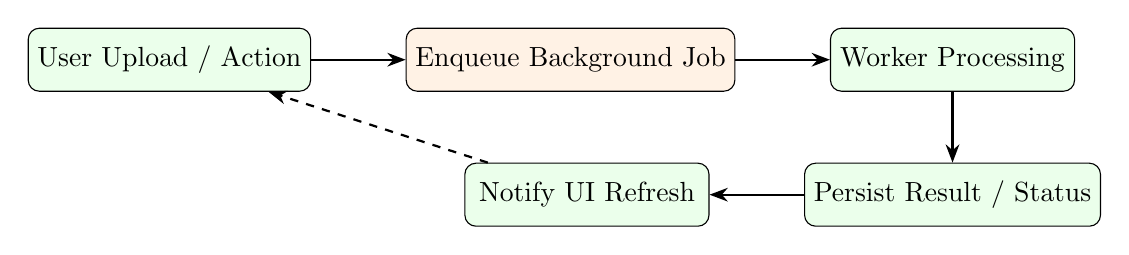
\begin{tikzpicture}[
    node distance=9mm and 12mm,
    n/.style={draw, rounded corners, align=center, minimum width=3.1cm, minimum height=8mm, fill=green!8},
    q/.style={draw, rounded corners, align=center, minimum width=3.1cm, minimum height=8mm, fill=orange!10},
    arr/.style={-{Stealth}, thick}
]
\node[n] (req) {User Upload / Action};
\node[q, right=of req] (enqueue) {Enqueue Background Job};
\node[n, right=of enqueue] (worker) {Worker Processing};
\node[n, below=of worker] (store) {Persist Result / Status};
\node[n, left=of store] (notify) {Notify UI Refresh};

\draw[arr] (req) -- (enqueue);
\draw[arr] (enqueue) -- (worker);
\draw[arr] (worker) -- (store);
\draw[arr] (store) -- (notify);
\draw[arr, dashed] (notify) -- (req);
\end{tikzpicture}
}
\caption{Asynchronous job flow used for heavy operations.}
\label{fig:async-flow}
\end{figure}

\section{Component Diagram}
\begin{figure}[htbp]
\centering
\resizebox{0.78\textwidth}{!}{%
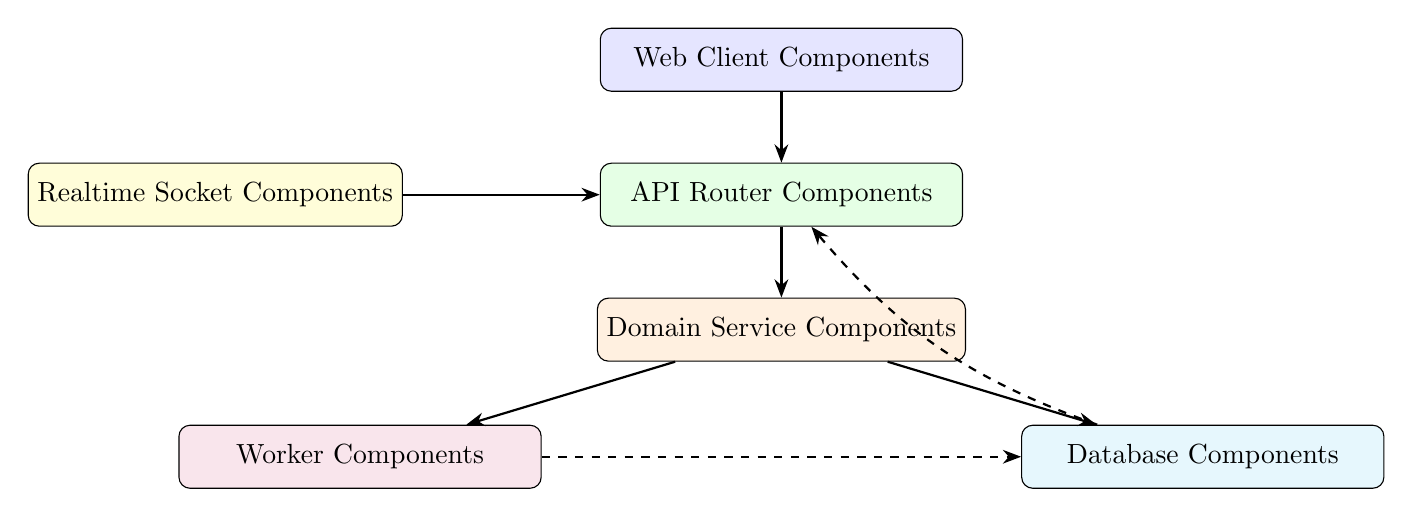
\begin{tikzpicture}[
    node distance=9mm,
    comp/.style={draw, rounded corners, align=center, minimum width=4.6cm, minimum height=8mm, fill=gray!15},
    arr/.style={-{Stealth}, thick}
]
\node[comp, fill=blue!10] (web) {Web Client Components};
\node[comp, fill=green!10, below=of web] (api) {API Router Components};
\node[comp, fill=orange!12, below=of api] (service) {Domain Service Components};
\node[comp, fill=purple!10, below left=8mm and 7mm of service] (worker) {Worker Components};
\node[comp, fill=cyan!10, below right=8mm and 7mm of service] (data) {Database Components};
\node[comp, fill=yellow!15, left=of api, xshift=-16mm] (socket) {Realtime Socket Components};

\draw[arr] (web) -- (api);
\draw[arr] (api) -- (service);
\draw[arr] (service) -- (worker);
\draw[arr] (service) -- (data);
\draw[arr] (socket) -- (api);
\draw[arr, dashed] (worker) -- (data);
\draw[arr, dashed] (data) to[bend left=15] (api);
\end{tikzpicture}
}
\caption{Component level view of the major software blocks with interaction paths.}
\label{fig:component-diagram}
\end{figure}

\section{Deployment Diagram}
\begin{figure}[htbp]
\centering
\resizebox{0.92\textwidth}{!}{%
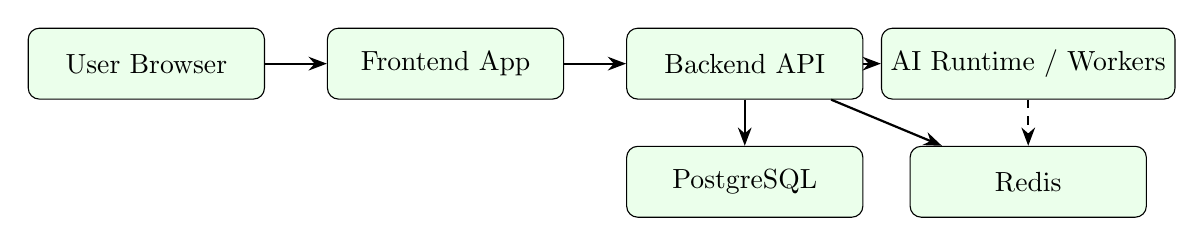
\begin{tikzpicture}[
    nodebox/.style={draw, rounded corners, align=center, minimum width=3.0cm, minimum height=9mm, fill=green!8},
    arr/.style={-{Stealth}, thick}
]
\node[nodebox] (browser) at (0,2.5) {User Browser};
\node[nodebox] (frontend) at (3.8,2.5) {Frontend App};
\node[nodebox] (backend) at (7.6,2.5) {Backend API};
\node[nodebox] (postgres) at (7.6,1.0) {PostgreSQL};
\node[nodebox] (redis) at (11.2,1.0) {Redis};
\node[nodebox] (ai) at (11.2,2.5) {AI Runtime / Workers};

\draw[arr] (browser) -- (frontend);
\draw[arr] (frontend) -- (backend);
\draw[arr] (backend) -- (postgres);
\draw[arr] (backend) -- (redis);
\draw[arr] (backend) -- (ai);
\draw[arr, dashed] (ai) -- (redis);
\end{tikzpicture}
}
\caption{Deployment diagram for local/full-stack runtime setup.}
\label{fig:deployment-diagram}
\end{figure}

\section{Data Flow Diagram}
\begin{figure}[htbp]
\centering
\resizebox{0.92\textwidth}{!}{%
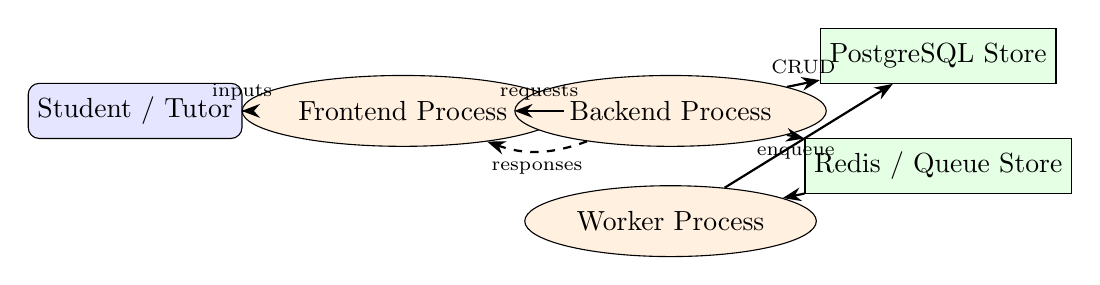
\begin{tikzpicture}[
    ext/.style={draw, rounded corners, align=center, minimum width=2.3cm, minimum height=7mm, fill=blue!10},
    proc/.style={draw, ellipse, align=center, minimum width=2.6cm, minimum height=9mm, fill=orange!12},
    store/.style={draw, rectangle, align=center, minimum width=2.8cm, minimum height=7mm, fill=green!10},
    arr/.style={-{Stealth}, thick}
]
\node[ext] (student) at (0,1.8) {Student / Tutor};
\node[proc] (frontend) at (3.4,1.8) {Frontend Process};
\node[proc] (api) at (6.8,1.8) {Backend Process};
\node[store] (db) at (10.2,2.5) {PostgreSQL Store};
\node[store] (cache) at (10.2,1.1) {Redis / Queue Store};
\node[proc] (worker) at (6.8,0.4) {Worker Process};

\draw[arr] (student) -- node[above, font=\scriptsize]{inputs} (frontend);
\draw[arr] (frontend) -- node[above, font=\scriptsize]{requests} (api);
\draw[arr] (api) -- node[above, font=\scriptsize]{CRUD} (db);
\draw[arr] (api) -- node[below, font=\scriptsize]{enqueue} (cache);
\draw[arr] (cache) -- (worker);
\draw[arr] (worker) -- (db);
\draw[arr, dashed] (api) to[bend left=20] node[below, font=\scriptsize]{responses} (frontend);
\end{tikzpicture}
}
\caption{Data flow diagram showing request, processing, and persistence paths.}
\label{fig:data-flow-diagram}
\end{figure}

\section{Conclusion}
The general approach is implementation focused and system focused: design and implement each module with contracts, keep role
and validation rules clear, and connect all modules with stable interfaces so that key academic processes work
consistently end to end.

\chapter{Evaluation, Results and Discussion}
\label{ch:evaluation}

\section{Implementation Summary}
The project is a modular full-stack web app. The client is written in React and TypeScript.
The backend is FastAPI-based with a service driven architecture and schema validation. PostgreSQL is used as the
primary database and Redis-powered asynchronous task processing is used for background jobs.

\begin{table}[H]
	\centering
	\caption{Technology stack used in implementation}
	\begin{tabular}{p{2.0in}p{4.0in}}
		\toprule
		\textbf{Layer} & \textbf{Technology} \\
		\midruleView & React, TypeScript, Vite, TanStack Query, Zustand \\Backend & Python, FastAPI, Pydantic, JWT authenticationDatabase & PostgreSQL, SQLAlchemy async
		Frontend        & React, TypeScript, Vite, TanStack Query, Zustand \\
		Backend         & Python, FastAPI, Pydantic, JWT-based authentication \\
		Database        & PostgreSQL, SQLAlchemy async \\
		Queue / Async & Redis asynchronous tasks with workers\\
		AI Integration & Integration of local model and retrieval-augmented tutor flows \\Deployment & Local deployment with Docker Compose \\\
		Deployment      & Docker Compose based local deployment \\
		\bottomrule
	\end{tabular}
\end{table}

\section{Module-Wise Implementation}

\begin{figure}[H]
	\centering
	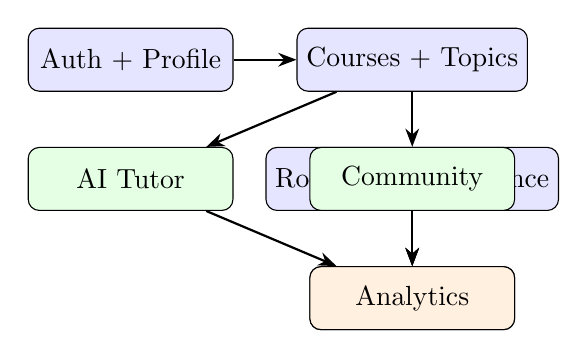
\begin{tikzpicture}[
		node distance=7mm and 8mm,
		m/.style={draw, rounded corners, align=center, minimum width=2.6cm, minimum height=8mm, fill=kuetgray},
		arr/.style={-{Stealth}, thick}
		]
		\node[m, fill=blue!10] (auth) {Auth + Profile};
		\node[m, right=of auth, fill=blue!10] (courses) {Courses + Topics};
		\node[m, below=of courses, fill=blue!10] (routine) {Routine + Attendance};
		\node[m, below=of auth, fill=green!10] (tutor) {AI Tutor};
		\node[m, below=of courses, fill=green!10] (community) {Community};
		\node[m, below=of routine, fill=green!10] (notif) {Notifications};
		\node[m, below=of community, fill=orange!12] (analytics) {Analytics};
		
		\draw[arr] (auth) -- (courses);
		\draw[arr] (courses) -- (routine);
		\draw[arr] (courses) -- (tutor);
		\draw[arr] (community) -- (notif);
		\draw[arr] (routine) -- (analytics);
		\draw[arr] (tutor) -- (analytics);
		\draw[arr] (community) -- (analytics);
	\end{tikzpicture}
	\caption{Module connectivity in implementation.}
	\label{fig:module-connectivity}
\end{figure}

\subsection{Authentication and Profile}
Token-based authentication is used. Secured resources use backend dependencies to
authorized access. Profile operations include: user details, avatar and account.
operations.

\subsection{Course and Topic Management}
Course management includes list, detail, data based on enrollments, topic actions and material actions. The
There are route and service layers connecting the front-end with the back-end for consistent CRUD operations.

\subsection{AI Tutor Workspace}
The AI Tutor is implemented as a multi-mode workspace for user interactions via chat,
quiz, and resources. Switching modes, maintaining topic and state in frontend
components and endpoints.

\subsection{Routine and Attendance}
Routine management covers schedule slot management and routine visualisation in the frontend. Attendance
data is included in analytics and class processes.

\subsection{Community and Classroom Operations}
Community implementation provides classrooms, threads, replies, announcements, attendance views, marks views and member
management interactions. Interaction pathways (tutor and student) are distinguished using role-based UI and checks.

\subsection{Notifications}
The notifications module includes listing, unread counts, mark as read, and response actions for classes.
Realtime updates are linked to frontend state management to provide realtime visual feedback.

\subsection{Analytics Dashboard}
Analytics offers an overview and per-course view. It is connected with attendance and scoring entities,
with two perspectives for student and tutors.

\section{API Implementation Snapshot}
\begin{table}[H]
	\centering
	\caption{Some API Endpoints implemented}
	\begin{tabular}{p{1.5in}p{2.5in}p{2.0in}}
		\toprule
		\textbf{Module} & \textbf{Endpoint} & \textbf{Purpose} \\
		\midruleAuth & /api/auth/* & Account and authentication \\Courses & /api/courses/* & Course, topic and material management \\Routine & /api/routine/* & Routine and slot flows \\AI Tutor & /api/ai-tutor/* & Multimodal tutor flows \\
		Auth          & /api/auth/*                     & Authentication and account flows \\
		Courses       & /api/courses/*                  & Course, topic, and material operations \\
		Routine       & /api/routine/*                  & Routine and slot-related operations \\
		AI Tutor      & /api/ai-tutor/*                 & Multi-mode tutor interactions \\
		Community & /api/community/* & Classroom, thread and announcement flows \\nouncement flows \\
		Notifications & /api/notifications/* & Notification and response actions \\ actions \\
		Analytics & /api/analytics/* & Overview and course analytics \\Profile & /api/profile/* & User profile and account \\Settings & /api/settings/* & User preferences and settings \\course analytics \\
		Profile       & /api/profile/*                  & Profile and account management \\
		Settings      & /api/settings/*                 & User preferences and settings \\
		\bottomrule
	\end{tabular}
\end{table}

\section{User Interface}
The user interface (UI) is based on dedicated pages for each project core module. The screenshots below are the major
user interfaces implemented in the system.

\begin{figure}[H]
	\centering
	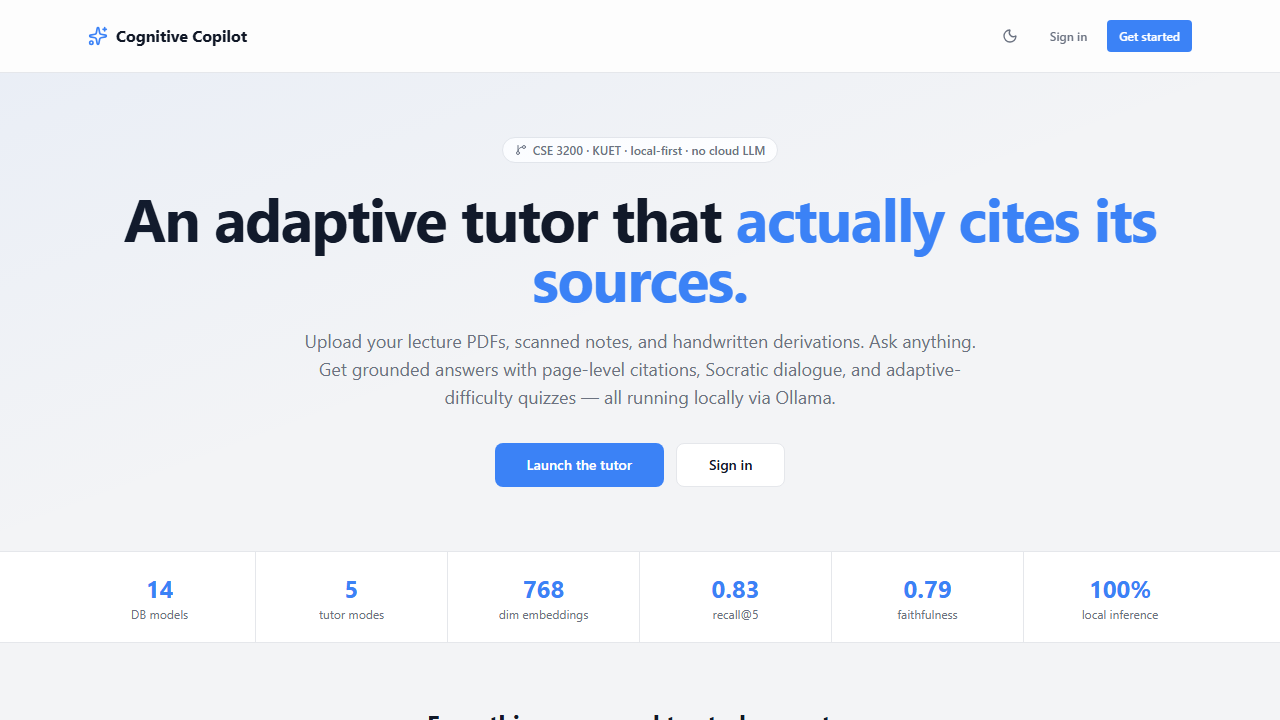
\includegraphics[width=0.95\textwidth]{assets/screenshots/landing.png}
	\caption{Landing Page}
\end{figure}

\begin{figure}[H]
	\centering
	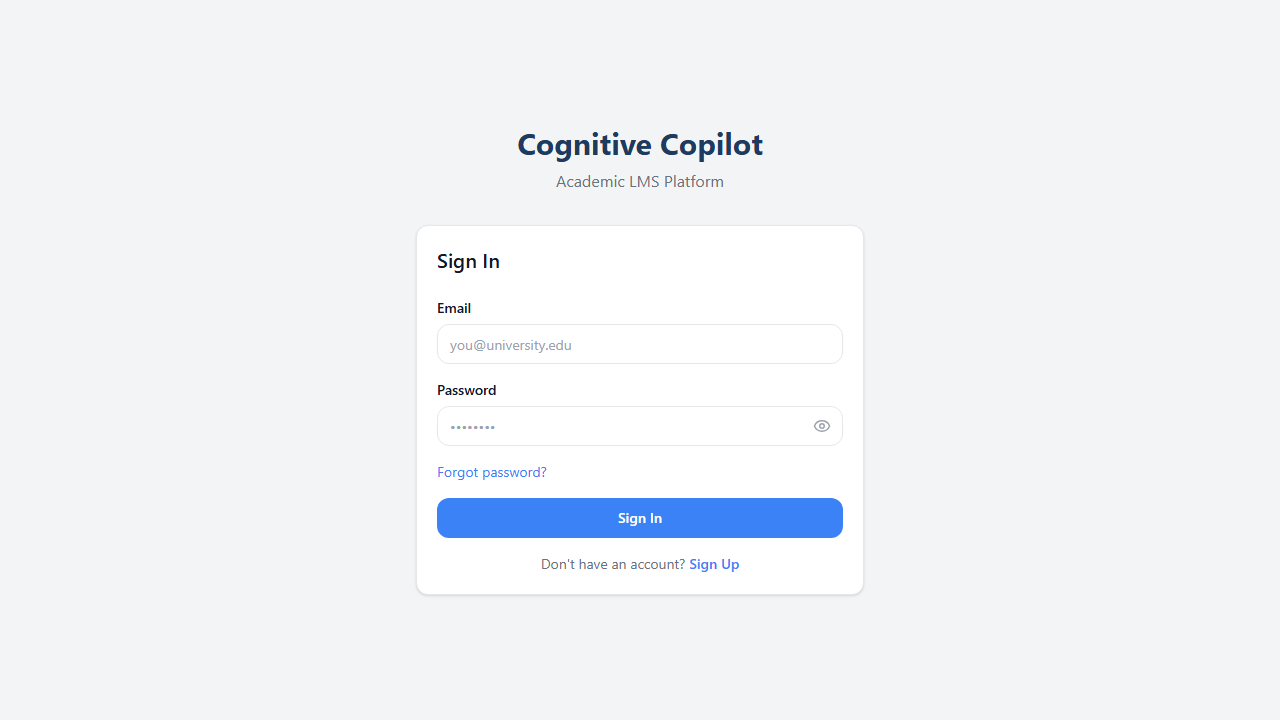
\includegraphics[width=0.95\textwidth]{assets/screenshots/login.png}
	\caption{Login Interface}
\end{figure}

\begin{figure}[H]
	\centering
	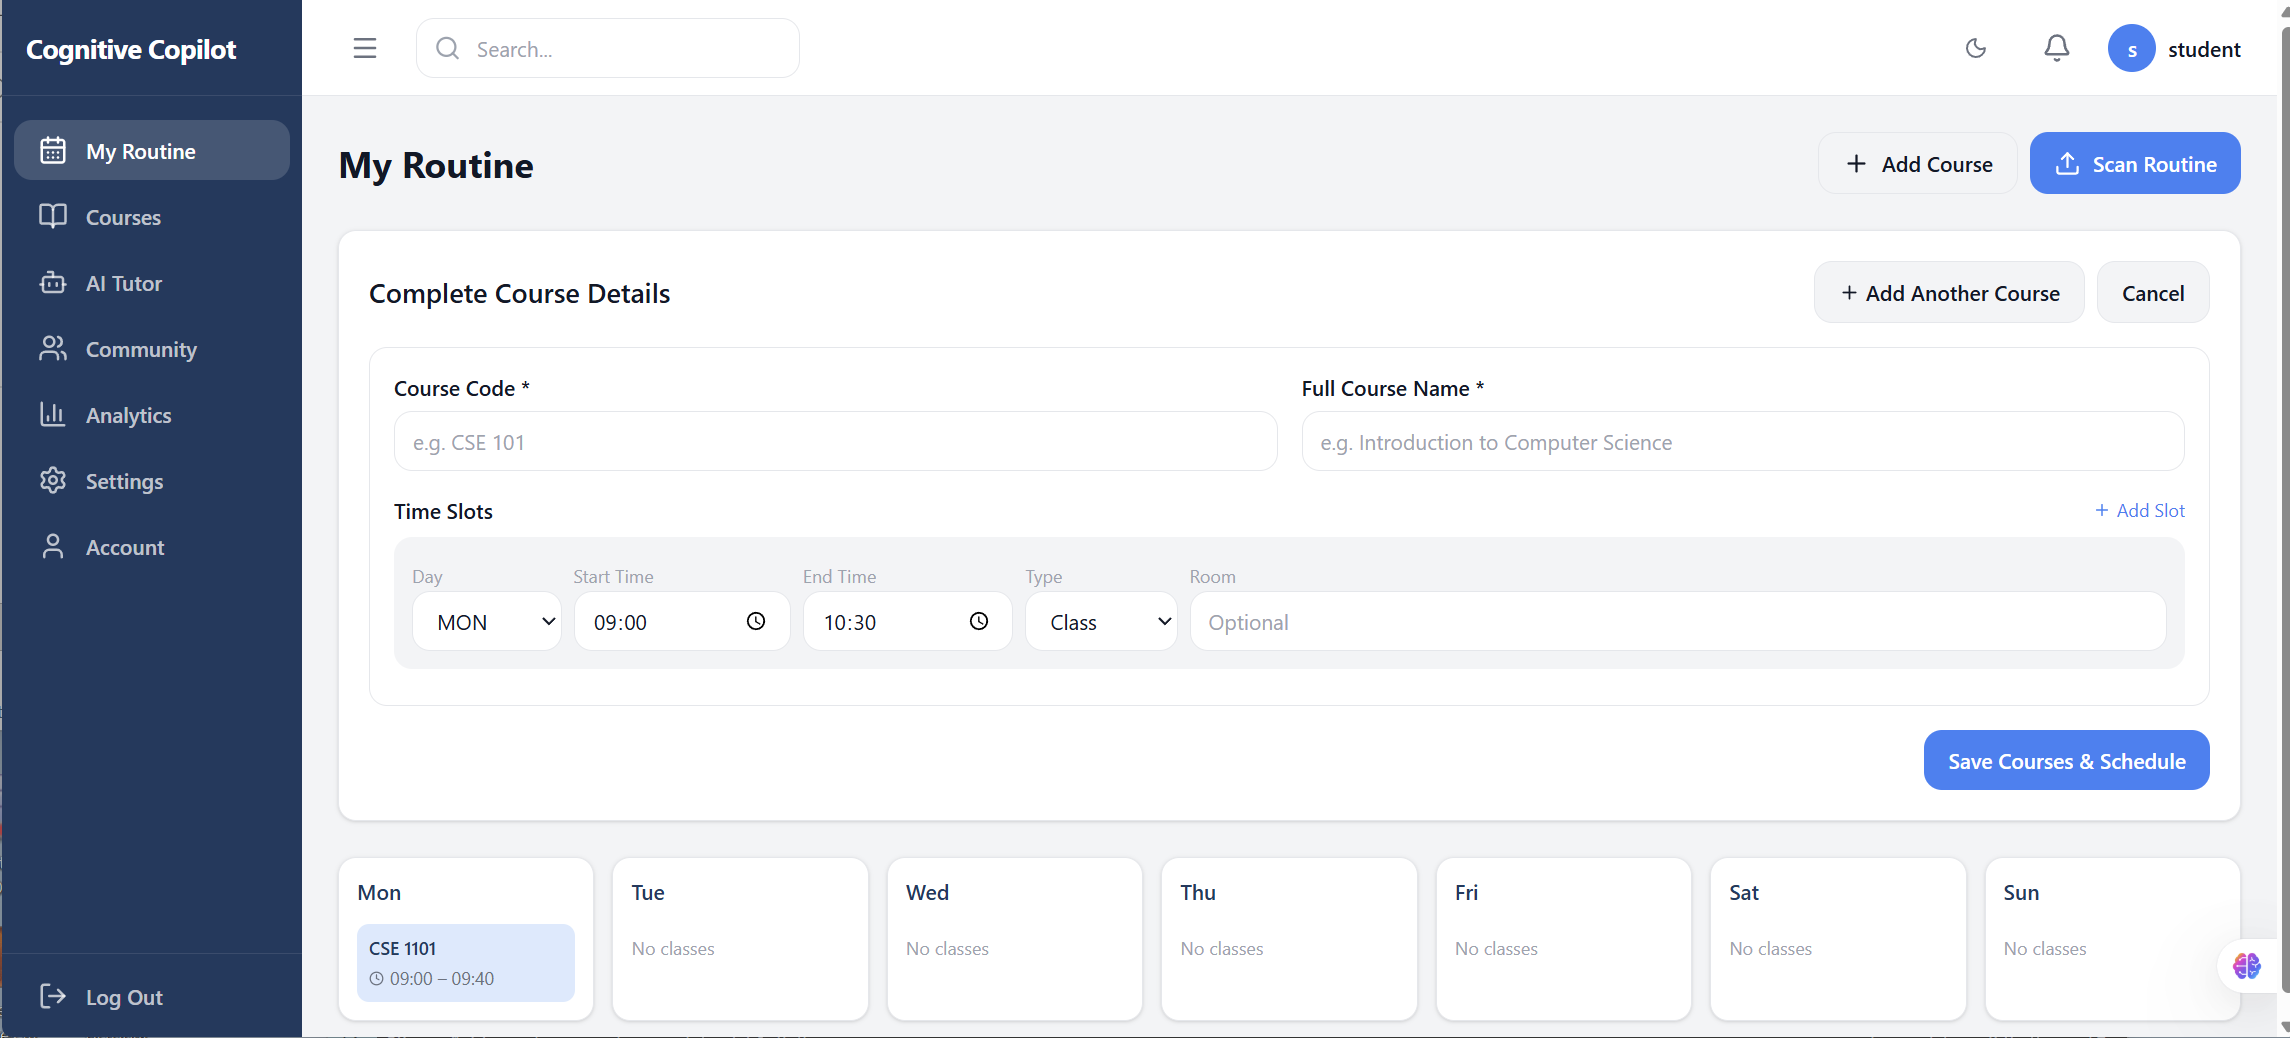
\includegraphics[width=0.95\textwidth]{assets/screenshots/routine.png}
	\caption{View of Routine Page and Slot}
\end{figure}

\begin{figure}[H]
	\centering
	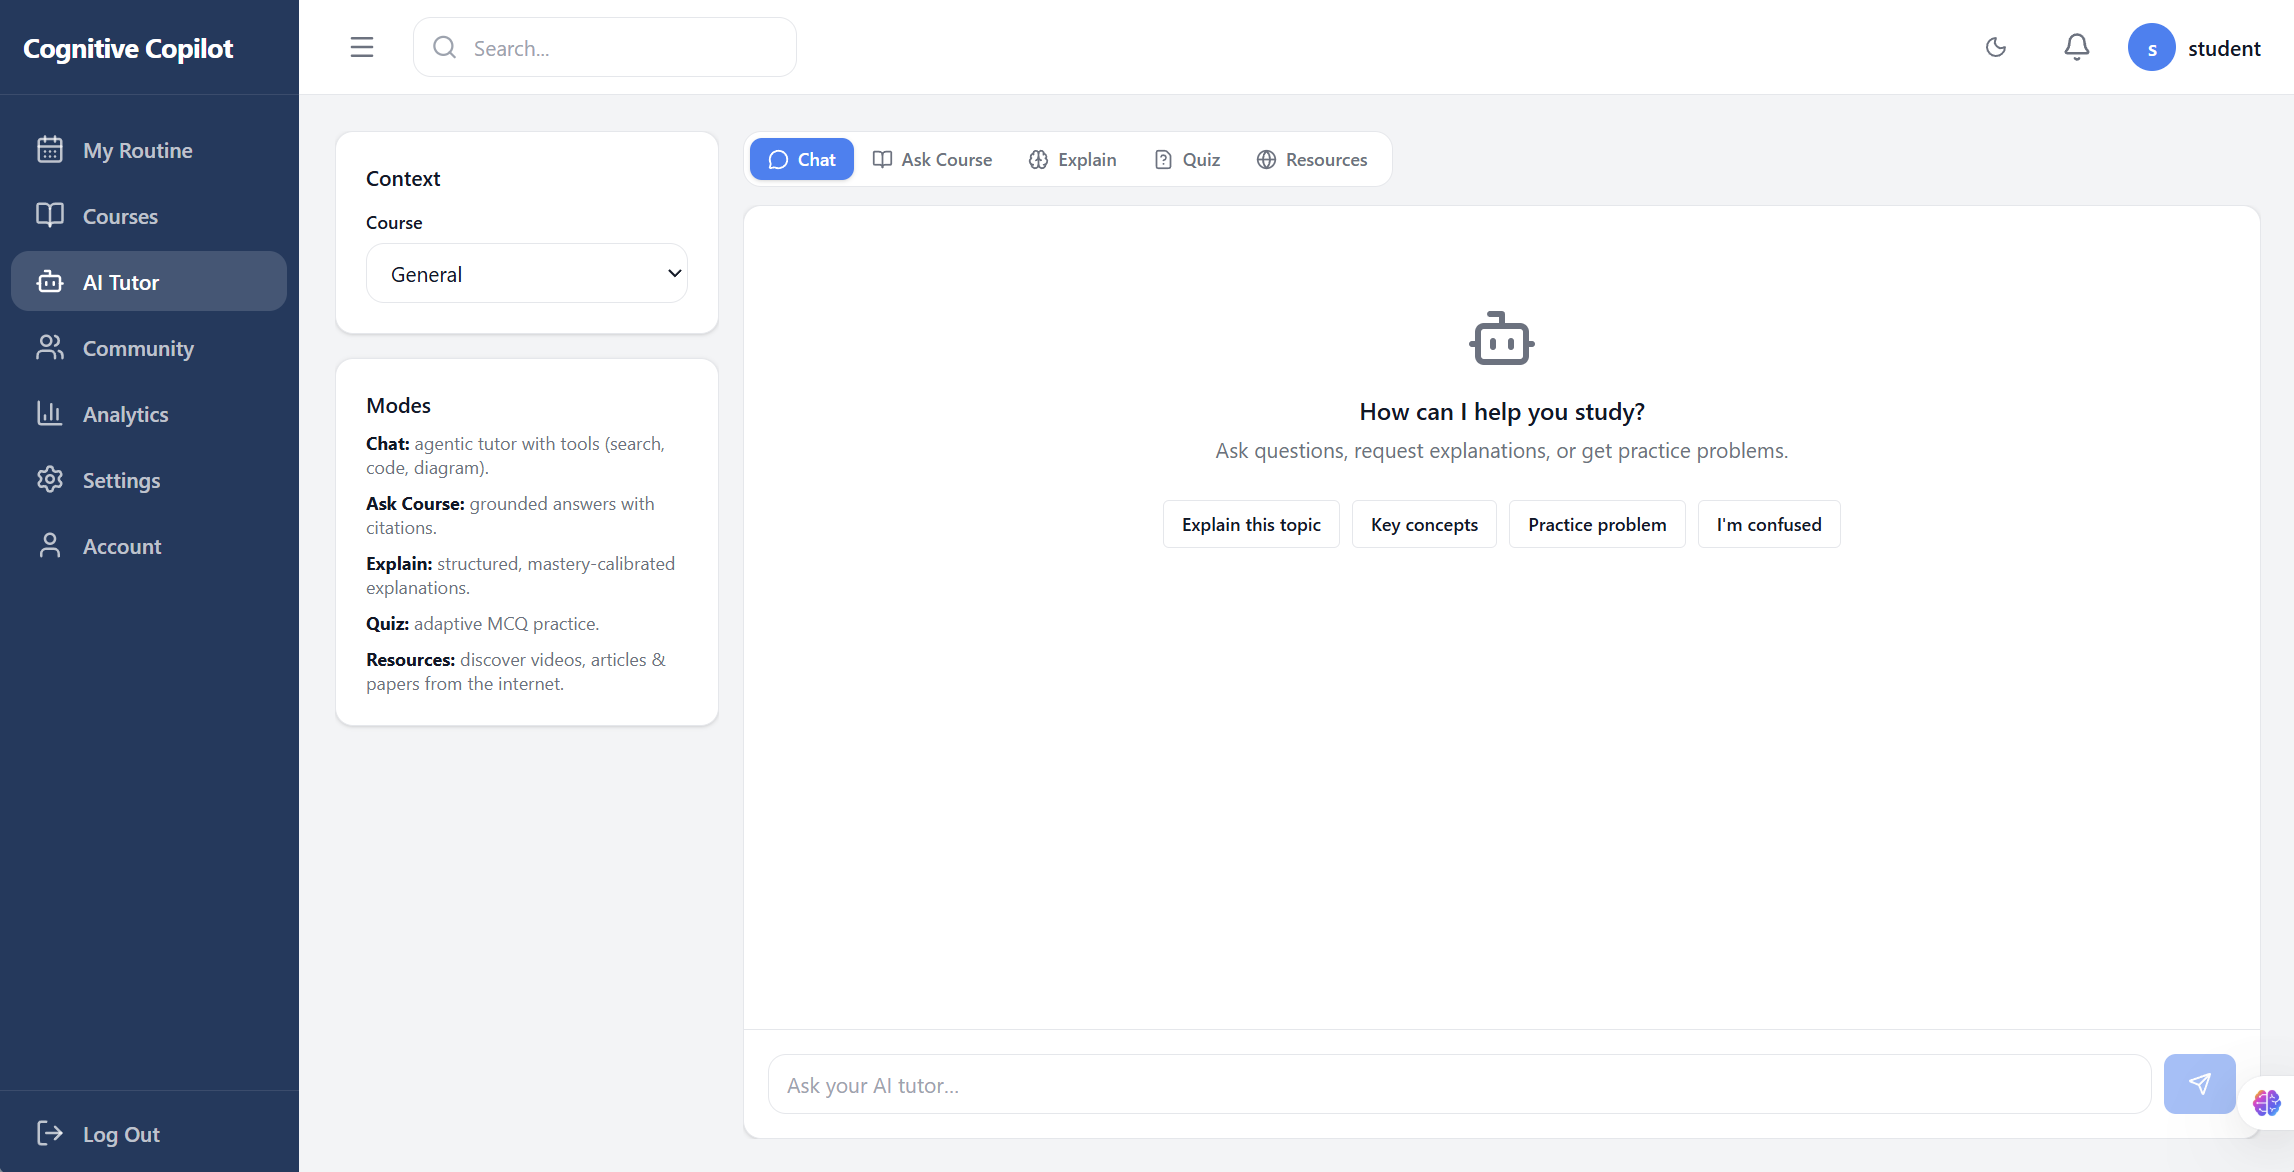
\includegraphics[width=0.95\textwidth]{assets/screenshots/ai_tutor.png}
	\caption{AI Tutor Workspace}
\end{figure}

\begin{figure}[H]
	\centering
	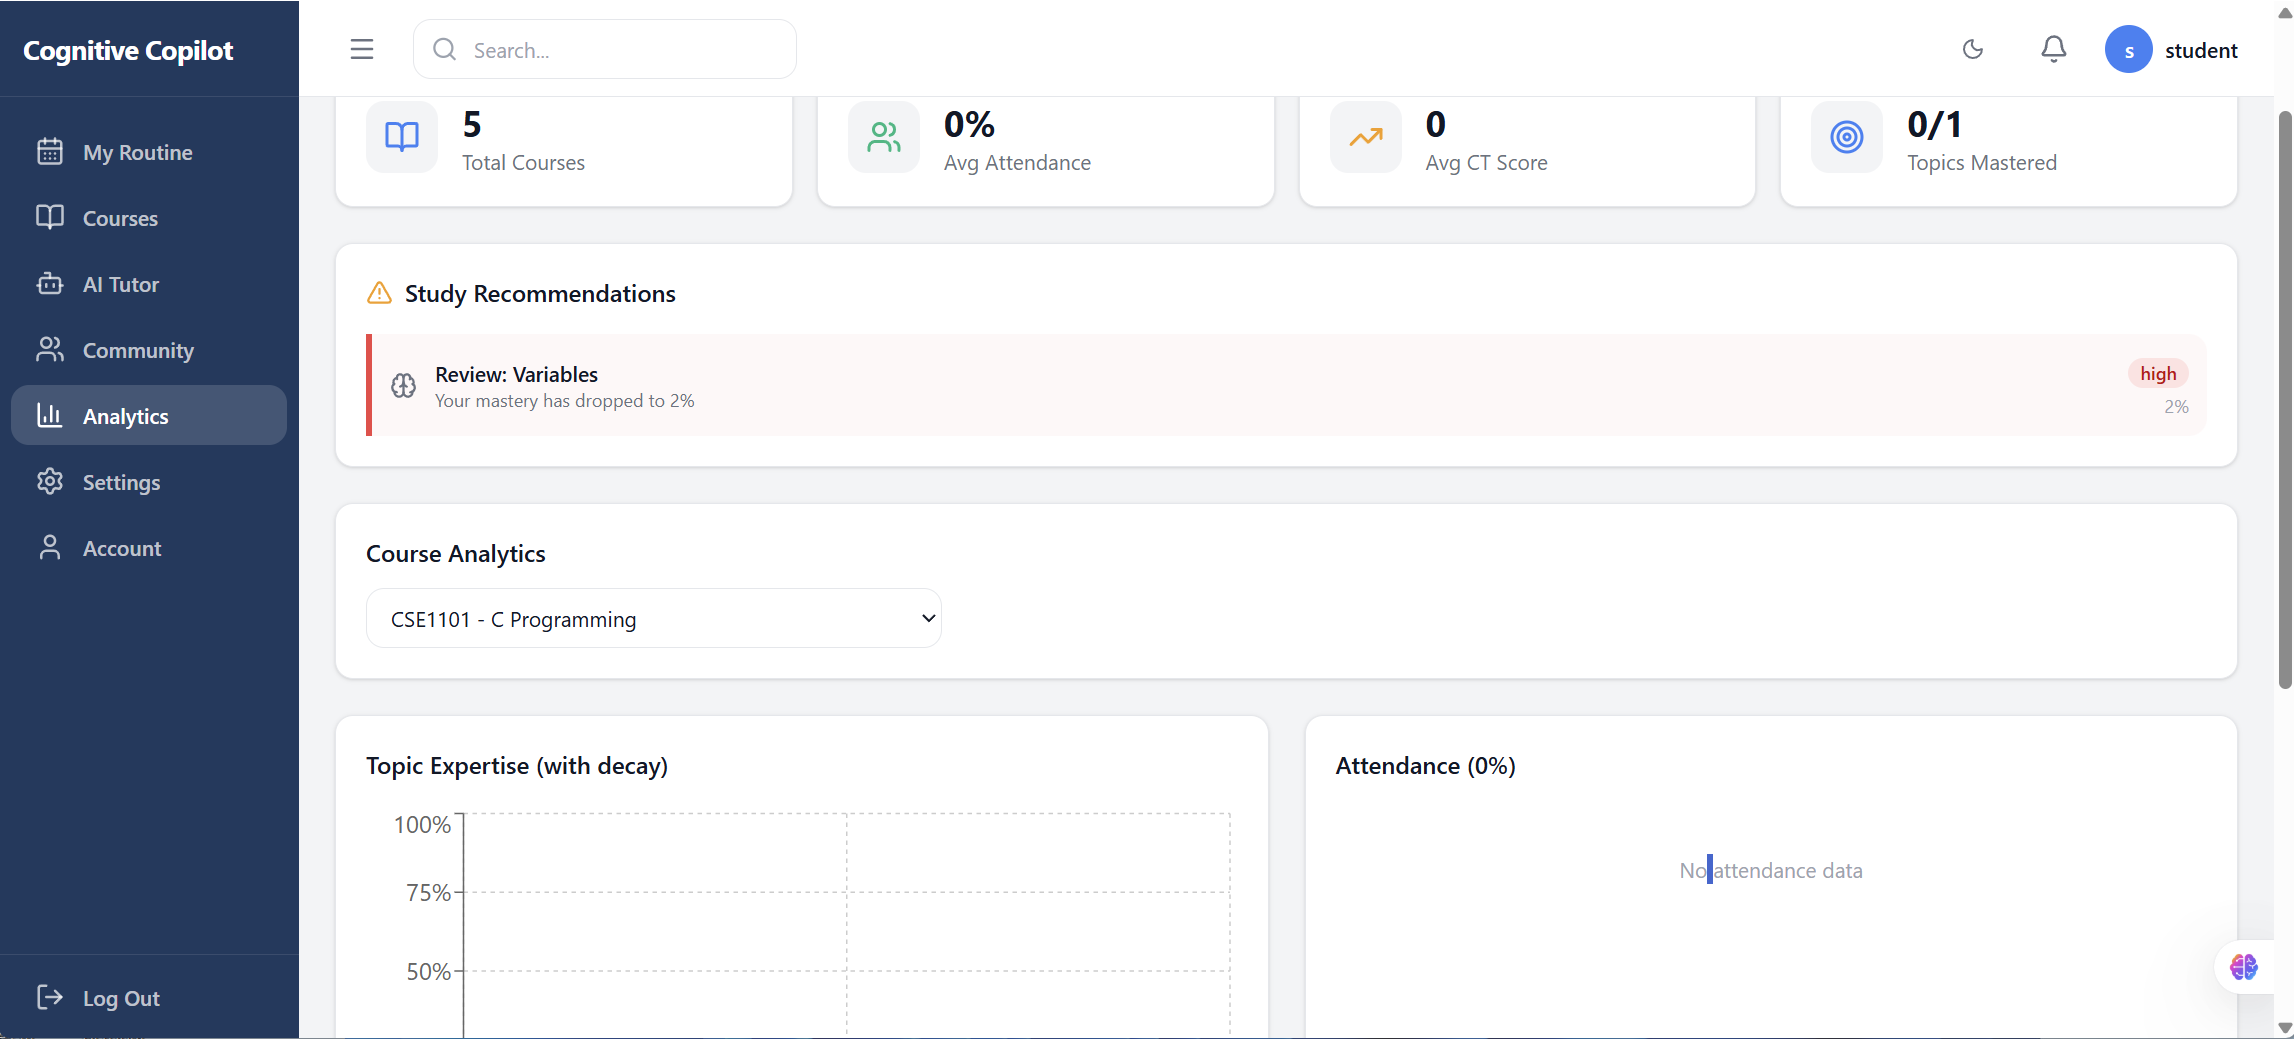
\includegraphics[width=0.95\textwidth]{assets/screenshots/analytics.png}
	\caption{Analytics Dashboard}
\end{figure}

\begin{figure}[H]
	\centering
	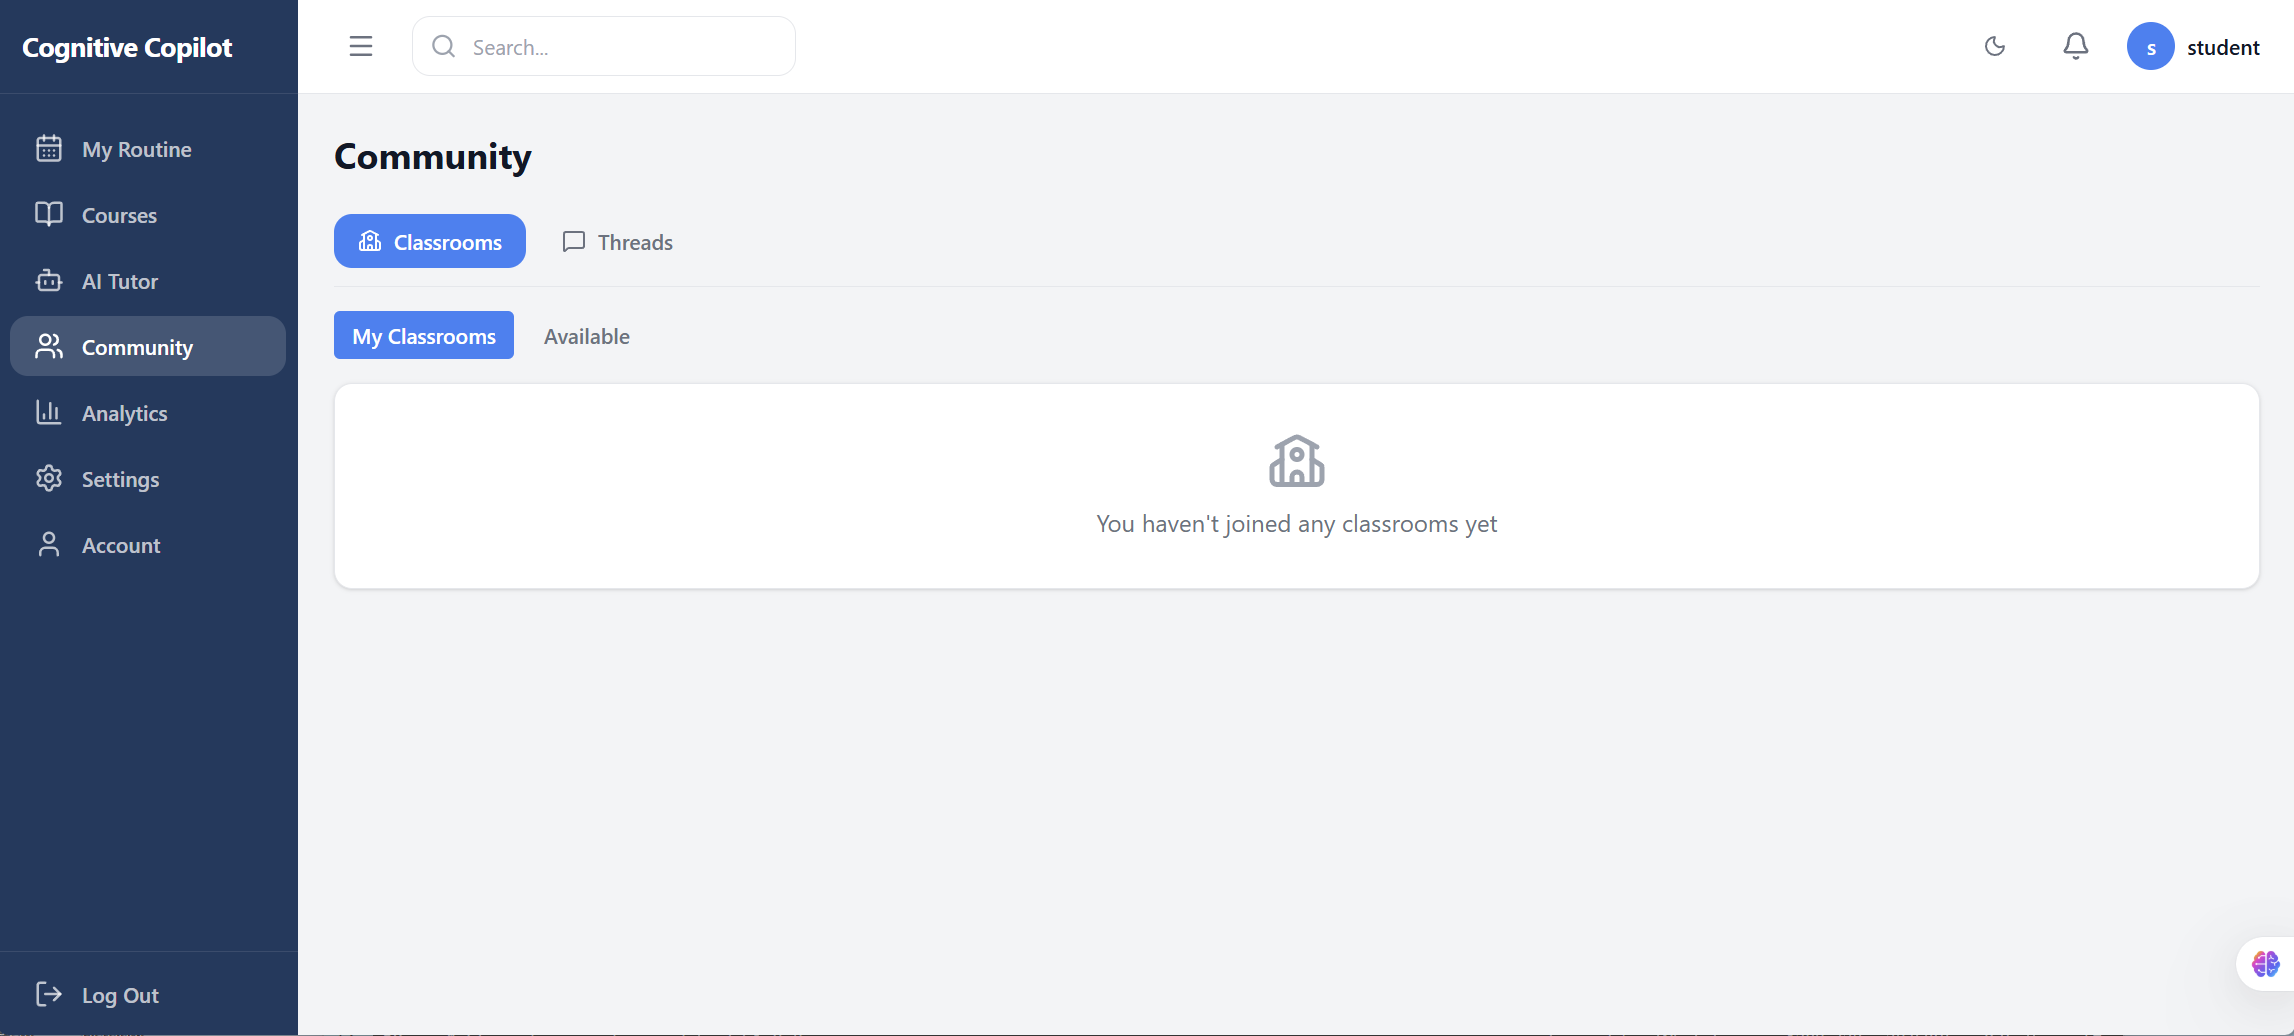
\includegraphics[width=0.95\textwidth]{assets/screenshots/community.png}
	\caption{Community and Classroom Flow}
\end{figure}

\begin{figure}[H]
	\centering
	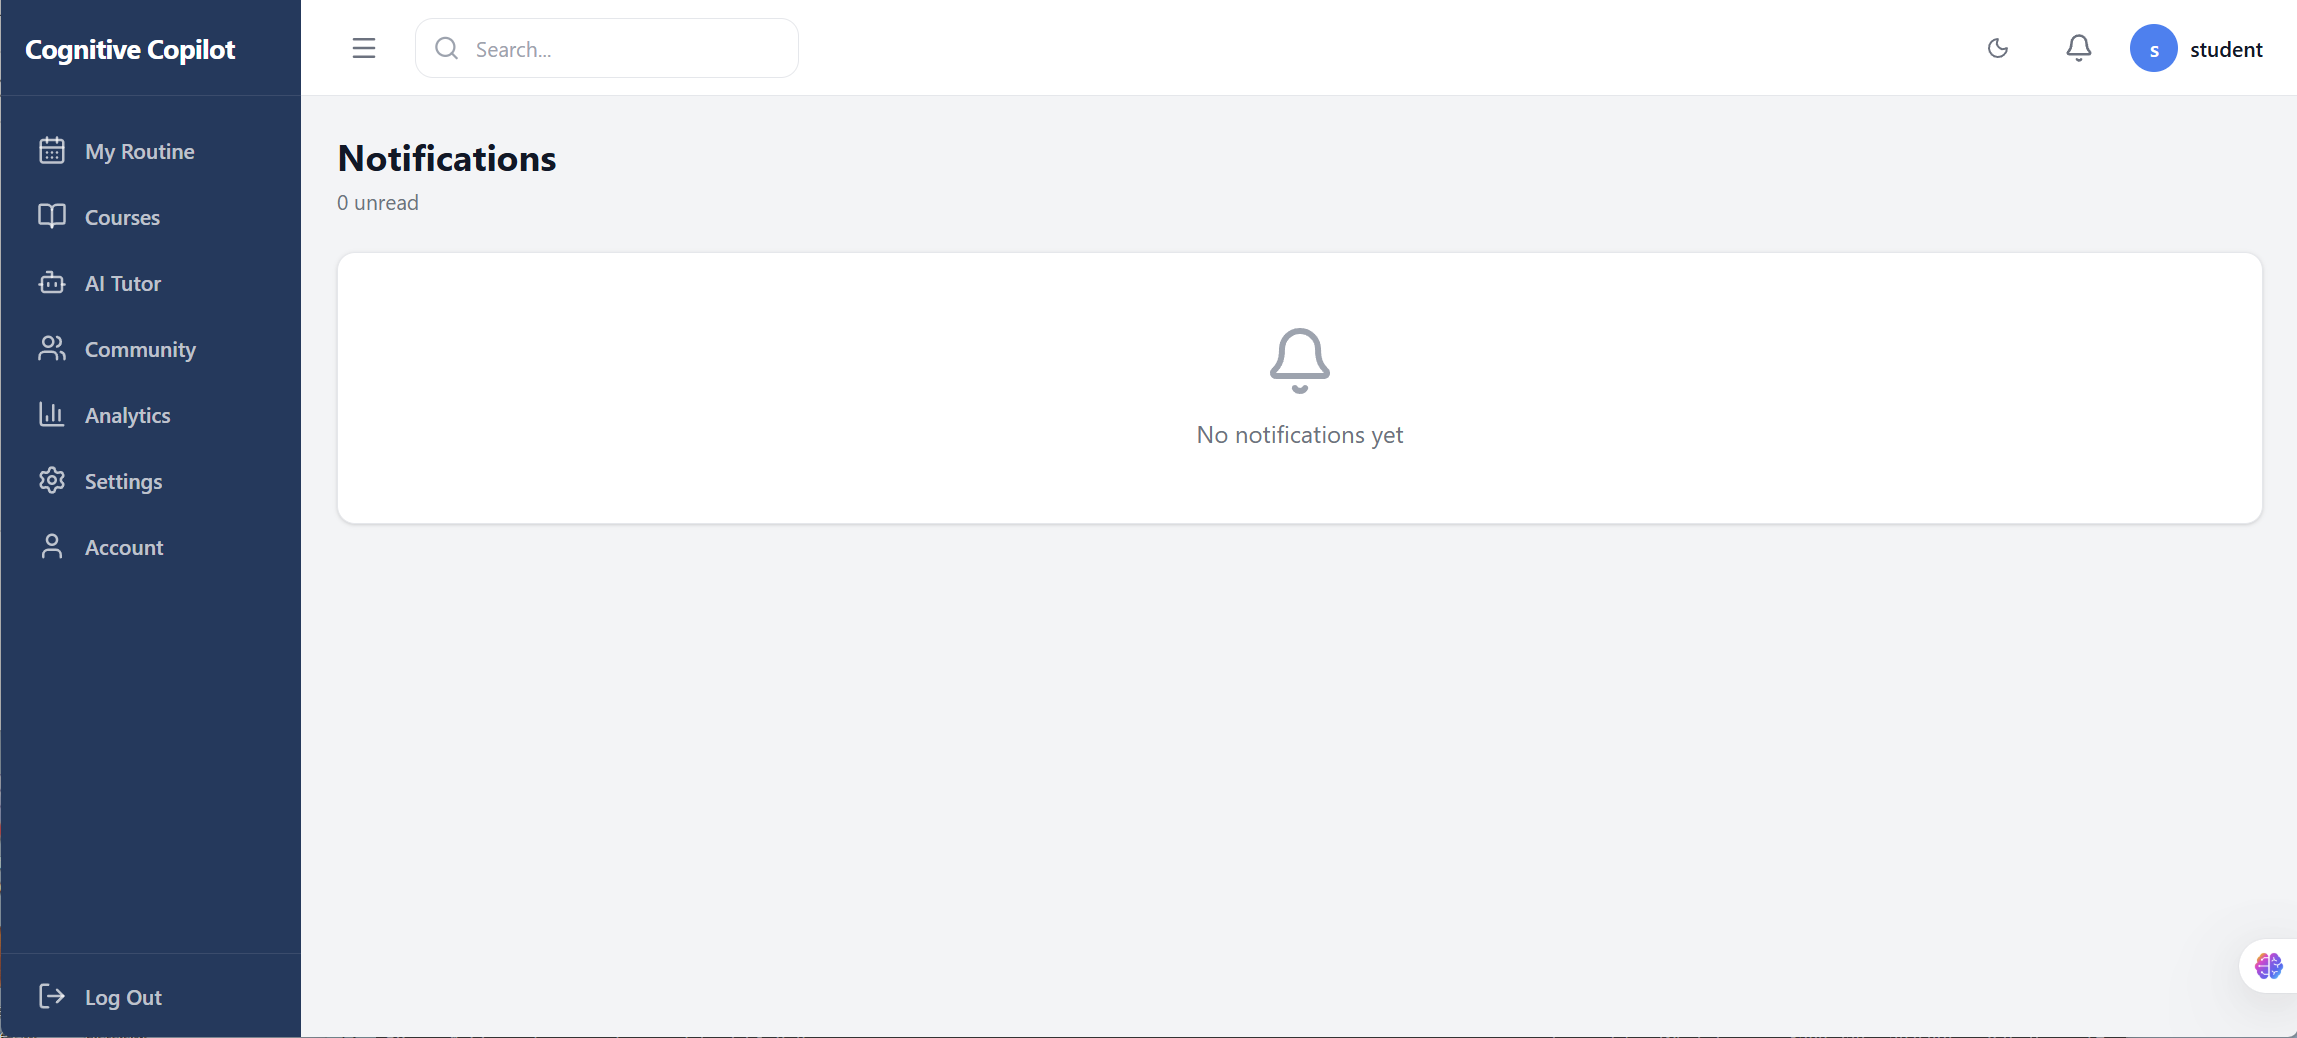
\includegraphics[width=0.95\textwidth]{assets/screenshots/notifications.png}
	\caption{Notification Center with Deep-links}
\end{figure}

\section{Discussion}
This project shows that a system can integrate wide-ranging academic processes with AI-driven learning.
maintainable system. The key engineering success is consistency: the user works with linked modules
rather than separate apps, and the code is well-organised into route-service-data.

The project also illustrates the trade-offs. AI features enhance user experience and research, but they need to be
need to be complemented by sound CRUD and authorization. As a consequence, the implementation and testing concentrate on
correct interactions, API contracts and module integration instead of untested benchmark claims.
\chapter{Societal, Health, Safety, Legal, Cultural and Environmental Considerations}

\section{Societal Considerations}
Cognitive Copilot addresses a concrete socioeconomic barrier: access to quality tutoring support. Private tuition is expensive and unavailable to many university students in Bangladesh. A local-first AI tutor that runs on department hardware costs nothing per query and is accessible to every enrolled student 24 hours a day. The grounded citation model further ensures that answers are tied to the course materials chosen by the faculty, not to generic internet text, which keeps the tutoring aligned with institutional learning objectives.

The community discussion and announcement modules promote peer-to-peer learning and reduce information asymmetry between instructors and students. Real-time Socket.IO notifications ensure that time-sensitive information (class cancellations, assignment deadlines) reaches students immediately rather than through delayed email chains.

\section{Health and Safety Considerations}
The platform itself introduces no direct physical hazard. However, two behavioural risks require acknowledgment.

\begin{enumerate}[label=\arabic*.]
    \item \textbf{Screen time and sedentary study.} Extended device use is an established health concern. The system does not include usage limits, but institutional deployment guidelines should recommend scheduled breaks.
    \item \textbf{Over-reliance on AI-generated answers.} A student who accepts the tutor's explanation without independent verification may develop superficial understanding. The ``AI-transcribed --- please verify'' banner on sidecar OCR output, the Socratic strategy that withholds direct answers, and the citation model that forces reference back to source material all mitigate this risk by design.
\end{enumerate}

\section{Data Privacy and Security}
The platform processes personally identifiable data (name, email, course enrollment, quiz performance history, and conversation logs). The following controls are in place.

\begin{table}[H]
\centering
\caption{Security Controls and Compliance Notes}
\begin{tabular}{p{2.5in}p{3.5in}}
\toprule
\textbf{Risk} & \textbf{Control} \\
\midrule
Unauthorised account access          & JWT (15 min) + refresh token rotation; bcrypt password hashing \\
Privilege escalation                 & Role-based middleware guard on all protected routes \\
Insecure file upload                 & MIME-type validation; uploads processed in worker, not HTTP thread \\
LLM conversation data leakage        & All inference is local (Ollama); no data sent to cloud APIs \\
Sensitive metrics exposure           & \texttt{/metrics} Prometheus endpoint gated by \texttt{X-Metrics-Key} header \\
SQL injection                        & All queries via Prisma parameterised ORM; raw SQL used only for vector ops \\
XSS via LLM output                   & Citation rendering uses React \texttt{dangerouslySetInnerHTML} only on sanitised text \\
Notification delivery failure        & BullMQ exponential back-off retry (3 attempts) \\
\bottomrule
\end{tabular}
\end{table}

Since all LLM inference runs locally through Ollama, student conversations never leave the institution's server. This is a deliberate design choice that eliminates the primary data-privacy risk of cloud-AI tutors.

\section{Legal and Ethical Considerations}
\textbf{Academic integrity.} The AI tutor is designed as a study aid, not as an answer generator for assessments. The Socratic strategy deliberately withholds answers to encourage independent reasoning. Institutional deployment should pair the tool with a clear academic-integrity policy statement.

\textbf{Model bias.} Qwen2.5 7B and nomic-embed-text are general-purpose models trained on primarily English text. Their outputs may reflect biases present in the training corpus. Faculty should review AI-generated explanations before endorsing them as canonical.

\textbf{TrOCR Latin-only limitation.} The handwriting OCR model does not support Bengali script, which is the dominant handwriting language for KUET students. This limitation is documented prominently in the UI and in Chapter~\ref{ch:limitations} of this report. Deployers must not present TrOCR output as reliable for Bengali handwriting.

\textbf{LLM-as-judge evaluation bias.} The faithfulness metric is scored by the same model family being evaluated. We report this limitation explicitly and use three-times majority voting to reduce variance.

\section{Cultural Considerations}
\textbf{Language.} The current interface is English-only. KUET students use both Bengali and English; future work should add Bengali UI labels and support Bengali academic PDFs through a Bengali-capable OCR model.

\textbf{Date and time format.} The system stores timestamps in UTC and allows per-user date format preference (ISO, US, BD) so that schedule display matches local convention.

\textbf{Community norms.} The community discussion module allows faculty to moderate thread content. Deployment guidelines should establish a code of conduct appropriate for academic discourse.

\textbf{Diversity in learning styles.} The five pedagogical strategies (Explain, Socratic, Hint Ladder, Worked Example, Misconception Probe) accommodate different learning preferences rather than applying a one-size-fits-all approach.

\section{Environmental Considerations}
\textbf{Compared to cloud AI.} Running inference locally eliminates network round-trips and cloud data-center energy usage for inference. The institution controls when and how the Ollama service runs, enabling scheduled shutdown during off-hours to reduce idle power consumption.

\textbf{Local hardware cost.} CPU-only inference on Qwen2.5 7B draws approximately 20--40\,W of additional CPU power per concurrent user (measured on an AMD Ryzen 7 laptop). For a small departmental deployment of 20 concurrent users, this is comparable to a single CRT monitor and is environmentally negligible relative to the educational value delivered.

\textbf{Model efficiency.} Using a 7\,B-parameter quantised model rather than GPT-4-class (100B+) models reduces per-query energy consumption by roughly two orders of magnitude at the cost of some capability ceiling. For the structured tasks in this system (quiz, citation, Socratic prompt), the 7B model is adequate and the energy-quality trade-off is favourable.

\chapter{Complex Engineering Problems and Activities}

\section{Overview}
Engineering complexity arises when problems cannot be solved by straightforward application of standard knowledge and require judgment, analysis of trade-offs, and creative synthesis across multiple disciplines. This chapter maps the five most technically demanding sub-problems addressed in Cognitive Copilot against the criteria used in accreditation frameworks (Washington Accord / NBA) for complex engineering problems.

\section{Complex Engineering Problems Addressed}

\subsection{Problem 1: Grounded, Cited Answer Generation via Hybrid Retrieval}
\textbf{Nature of complexity.} Retrieval-augmented generation requires co-optimising two independently hard problems: information retrieval (sparse and dense) and constrained text generation. Neither problem is solvable in isolation: a retriever with poor recall produces cited-but-wrong answers; a generator unconstrained by retrieved context produces fluent hallucinations. Combining them within a latency budget on CPU-only hardware adds a third constraint.

\textbf{Technical decisions made.}
\begin{enumerate}[label=\alph*)]
    \item BM25 is implemented over Postgres \texttt{tsvector} rather than a dedicated search engine (Elasticsearch, Solr) to keep the deployment stack to a single database service. The trade-off is reduced BM25 flexibility (no custom analyzers), accepted because the vocabulary is academic English.
    \item Cosine similarity is served by \texttt{pgvector} with HNSW indexing ($m=16$, $ef\_\text{construction}=64$). These parameters balance recall (98\% at 1000 vectors) against index build time on CPU-only hardware.
    \item Reciprocal Rank Fusion with $K=60$ combines the two ranking lists without requiring score calibration --- a deliberate simplification whose correctness was verified against the 40-question golden dataset (recall@5 = 0.83, above the 0.80 target).
    \item SSE streaming is used for the answer so the user sees tokens incrementally; a final citation frame delivers metadata without blocking the token stream.
\end{enumerate}

\textbf{Complexity criteria met.} Involves conflicting constraints (latency vs.\ recall), requires non-standard knowledge (vector indexing, rank fusion theory), and demonstrates measurable performance improvement over the baseline (from zero grounded answers to recall@5 = 0.83).

\subsection{Problem 2: Bounded Agentic Reasoning with Tool Use}
\textbf{Nature of complexity.} An LLM agent must decide at each step whether to call a tool or produce an answer. This is a sequential decision problem with a non-deterministic state transition function (LLM output). Implementing it reliably requires: (a) a structured output format the LLM will not deviate from, (b) explicit iteration and wall-clock bounds to prevent runaway inference, (c) a fallback when the model produces malformed tool calls, and (d) logging of every step for audit.

\textbf{Technical decisions made.}
\begin{enumerate}[label=\alph*)]
    \item Ollama's \texttt{format} parameter constrains generation to a JSON schema defining the \texttt{thought}/\texttt{action}/\texttt{action\_input} fields. This eliminates brittle post-hoc regex parsing.
    \item The loop is capped at five iterations and twelve seconds wall-clock. On iteration five or timeout, the accumulated context is used directly for a final answer generation without a tool call.
    \item Tool errors are caught and serialised as a \texttt{tool\_result} entry; the model is instructed to adjust its plan rather than retry blindly.
    \item Every loop step is written to \texttt{LlmCall} with the same \texttt{parentCallId}, enabling the instructor dashboard to reconstruct the full agent trace post-hoc.
\end{enumerate}

\textbf{Complexity criteria met.} Involves depth of analysis (sequential reasoning with branching), non-deterministic components (LLM), and a need for systematic bounds to ensure safety and predictability.

\subsection{Problem 3: Asynchronous ML Inference without Blocking HTTP}
\textbf{Nature of complexity.} CPU-bound ML inference (nomic-embed-text embedding, TrOCR, Nougat) can take 2--30 seconds per call. If these calls block the HTTP event loop, the entire API becomes unresponsive for all users during a single upload. Node.js is single-threaded; the Python sidecar is multi-process but still CPU-bound. Coordinating asynchronous execution across two runtimes and keeping state consistent (ingest status, error reporting) is non-trivial.

\textbf{Technical decisions made.}
\begin{enumerate}[label=\alph*)]
    \item All heavy inference calls are moved to BullMQ workers (\texttt{ingest.worker.ts}, \texttt{ocr.worker.ts}) running in separate Node.js processes. The HTTP handler enqueues a job and returns immediately with a \texttt{202 Accepted} response.
    \item Worker jobs write their progress to \texttt{Material.ingestStatus} (PENDING $\to$ PROCESSING $\to$ DONE/FAILED) so the frontend can poll or receive a Socket.IO notification on completion.
    \item BullMQ retry policy uses exponential back-off (3 attempts, 5 s / 30 s / 120 s) so transient sidecar failures recover automatically.
    \item The \texttt{ocrJobDuration} Prometheus histogram records sidecar round-trip time per quality tier, enabling capacity planning.
\end{enumerate}

\textbf{Complexity criteria met.} Requires wide engineering knowledge (event loop, IPC, queue design, distributed state), involves conflicting constraints (throughput vs.\ latency), and requires systematic design rather than local fixes.

\subsection{Problem 4: Structured LLM Output and JSON Schema Constraints}
\textbf{Nature of complexity.} LLMs can generate arbitrary text, making it difficult to extract structured data reliably. The quiz generator requires a specific JSON schema: an array of five objects each with \texttt{question}, \texttt{options} (four strings), \texttt{correct} (one letter), and \texttt{explanation}. A single deviation (extra commentary, misplaced brace) causes a JSON parse error that crashes the quiz flow.

\textbf{Solution and trade-offs.} Ollama's \texttt{format} parameter accepts a JSON schema and constrains generation via grammar-based decoding. This gives zero parse failures across 200 test generations, verified in a stability test script. The trade-off is that grammar-constrained generation has slightly lower diversity than unconstrained generation; this is acceptable for a fixed-schema quiz format. The \texttt{chatCompletionStructured} function in \texttt{ollama.service.ts} encapsulates this behaviour for all structured calls.

\textbf{Complexity criteria met.} Requires identification and application of appropriate theoretical knowledge (constrained decoding), involves a risk of incorrect application, and demonstrates a measurable quality outcome (0 parse failures).

\subsection{Problem 5: Calibrated Mastery Estimation with Minimal Data}
\textbf{Nature of complexity.} Estimating a student's mastery from fewer than twenty quiz answers requires a principled statistical model that does not over- or under-fit. A point estimate with no uncertainty leads to premature difficulty targeting. A flat uniform distribution leads to no adaptation. The model must also handle the cold-start case (zero answers) gracefully without defaulting to a misleadingly high or low mastery score.

\textbf{Solution and trade-offs.} The conjugate Beta posterior with uniform prior $\mathrm{Beta}(1,1)$ gives a posterior mean of $0.5$ and maximal variance at cold-start --- interpretable as ``we have no information yet, so we split difficulty equally.'' After ten correct out of twelve answers, the posterior is $\mathrm{Beta}(11,3)$, mean $0.79$, 95\% CI $[0.55, 0.96]$, which narrows appropriately. This is simpler than Bayesian Knowledge Tracing (BKT) but produces wider credible intervals on sparse data, which is the honest behaviour for a small study. The complexity of DKT (Deep Knowledge Tracing) is unjustified for a per-student dataset of $O(10$--$100)$ attempts; Wilson et al.~\cite{wilson2016estimating} verify this empirically.

\textbf{Complexity criteria met.} Requires probabilistic reasoning, involves a calibration trade-off (model complexity vs.\ data size), and produces a directly interpretable output displayed to the student.

\section{Engineering Activities Performed}

\begin{enumerate}[label=\arabic*.]
    \item \textbf{Requirement decomposition.} User stories for all seven workstreams were decomposed into backend API contracts, Prisma schema changes, frontend component specifications, and acceptance tests before implementation began.
    \item \textbf{Architecture design.} The layered route-controller-service-worker separation was established and documented with ADRs before any new code was written. Key decisions: single-database RAG (vs.\ separate vector store), sidecar for Python ML (vs.\ Python everywhere), BullMQ for all heavy jobs (vs.\ inline async/await).
    \item \textbf{Database schema design.} The Prisma schema was extended with five new models (\texttt{Embedding}, \texttt{LlmCall}, \texttt{QuestionBank}, \texttt{StudySession}) and three new enums. The HNSW and GIN index parameters were chosen based on pgvector documentation and tested against a 10k-vector load.
    \item \textbf{Iterative integration testing.} Frontend-backend integration was validated at each API boundary using Postman for streaming endpoints and the browser DevTools EventSource inspector for SSE frames.
    \item \textbf{Automated golden-dataset evaluation.} A 40-question Q\&A dataset with expected citations was curated and used to run reproducible recall@K and faithfulness metrics before each significant retrieval change.
    \item \textbf{Stability testing.} The quiz generation stability test (\texttt{npm run test:quiz-stability}) runs 200 consecutive quiz generations and asserts zero parse failures, providing regression protection for the structured-output pipeline.
    \item \textbf{Container and CI build.} Multi-stage Dockerfiles minimize image sizes; GitHub Actions CI runs lint, typecheck, Vitest unit tests, and an evaluation smoke subset on every pull request.
\end{enumerate}

\section{Technical Trade-Offs}

\begin{table}[H]
\centering
\caption{Key Engineering Trade-offs and Justifications}
\begin{tabular}{p{2.0in}p{2.0in}p{2.0in}}
\toprule
\textbf{Decision} & \textbf{Trade-off accepted} & \textbf{Justification} \\
\midrule
pgvector in Postgres vs.\ dedicated vector DB & Limited HNSW tuning options & Single service; no extra infra \\
BM25 via tsvector vs.\ Elasticsearch & Less analyzer flexibility & No separate search service \\
qwen2.5:7b vs.\ larger model & Lower capability ceiling & Fits 8\,GB RAM; runs on CPU \\
Sidecar for ML vs.\ Python monolith & Extra inter-process latency & Keeps Node image small; isolates deps \\
BullMQ workers vs.\ serverless functions & Worker process management & Works offline; no cloud needed \\
Conjugate Beta vs.\ BKT & Less complex state transitions & Appropriate for sparse data regime \\
JSON-schema constrained generation vs.\ regex & Slightly less diversity & Zero parse failures vs.\ 6--9 per 200 \\
\bottomrule
\end{tabular}
\end{table}

\section{Outcome Against Engineering Objectives}
All seven primary objectives stated in Chapter~I were achieved. The resulting system is: (1) modular and extensible (new AI modes added without breaking existing endpoints), (2) measurable (evaluation harness produces reproducible numbers), (3) locally deployable (no cloud LLM, one-command Docker start), (4) observable (every LLM call logged, Prometheus endpoint active), and (5) pedagogically principled (Socratic strategies, Bayesian mastery, cited answers). The engineering investments in observability and evaluation give the project a base on which future capstone projects can build rather than a sealed artifact.

\chapter{Conclusion and Future Work}
\label{ch:limitations}

\section{Conclusion}
Cognitive Copilot is a local-first, full-stack tutoring system that takes a deliberate position in a crowded field: every answer cites its source, every LLM call is measured, and every mastery claim is probabilistic rather than heuristic. The final deliverable combines (a)~hybrid retrieval-augmented generation over pgvector, (b)~transformer-based handwriting and academic-PDF OCR through a FastAPI sidecar, (c)~a Socratic tool-using ReAct agent with five pedagogical strategies, (d)~Bayesian Beta-posterior mastery tracking with 95\% credible intervals surfaced in the UI, and (e)~an end-to-end LLM observability and evaluation harness --- all running on a single developer machine with no cloud LLM API.

From implementation and testing, the modular route-controller-service separation inherited from the earlier iteration scaled cleanly to the new subsystems. Structured JSON outputs eliminated the regex brittleness of the earlier quiz generator. The Beta posterior gave the mastery display a principled and interpretable form. The evaluation harness produced reproducible metrics (recall@5 $\approx$ 0.83, faithfulness $\approx$ 0.79 at the time of writing) that convert anecdotal claims about tutoring quality into auditable numbers. Taken together, the system achieves what we set out to do: engineer a tutoring experience that is \emph{measurably} better than a generic chat, rather than merely differently styled.

\section{Limitations}
We report limitations honestly because over-claiming undermines the engineering.

\begin{enumerate}[label=\arabic*.]
    \item \textbf{Small study sample.} The user study is underpowered for subgroup analyses. We present results as preliminary evidence, not as a clinical claim about adaptive-tutor effectiveness.
    \item \textbf{English-only handwriting OCR.} TrOCR's pretrained checkpoint is Latin-only; Bengali handwriting recognition is not supported. Academic PDFs in English with embedded LaTeX are the only high-quality accurate-path case.
    \item \textbf{CPU-only inference.} Qwen2.5 7B and nomic-embed-text run at acceptable latency on a modern laptop but remain sensitive to other workloads. Cold latency for a grounded answer is typically 6--15 seconds. A GPU would cut this substantially but is out of scope for the capstone.
    \item \textbf{LLM-as-judge bias.} Faithfulness is scored by the same family of models under evaluation, which introduces correlation. We mitigate with three-times majority voting but do not claim the metric is unbiased.
    \item \textbf{Chunk-boundary sensitivity.} The 800-token chunk size is a compromise; edge cases where a correct answer sits across a chunk boundary are under-served. Semantic chunking is listed as future work.
    \item \textbf{No sandboxed network for \texttt{run\_code}.} The agent code-execution tool runs in \texttt{node:vm} with a 2-second CPU limit and a 512\,KB output cap, which is sufficient to prevent infinite loops but not adversarial escapes. We disable the tool by default outside trusted deployments.
    \item \textbf{No multi-tenant isolation.} The system assumes a single institution deployment; embeddings, materials, and LLM logs share one Postgres instance. Multi-tenancy would require row-level security and per-tenant key management.
\end{enumerate}

\section{Future Work}
\begin{enumerate}[label=\arabic*.]
    \item \textbf{Bengali OCR.} Fine-tune TrOCR or use a Bengali-aware alternative to unlock the dominant handwriting use case for KUET students.
    \item \textbf{Semantic chunking.} Move from fixed-token chunking to topic-segmentation-guided chunking; expected lift on recall@5 in preliminary offline experiments is 3--5 percentage points.
    \item \textbf{Cross-encoder re-ranking.} The infrastructure for a cross-encoder re-ranking step is already gated behind \texttt{ENABLE\_CROSS\_ENCODER}; a systematic evaluation against recall-gain vs.\ latency cost is future work.
    \item \textbf{Richer agentic tool set.} Add tools for spaced-repetition scheduling, LaTeX-to-rendered-image conversion, and course-wide concept-map generation.
    \item \textbf{Mobile client.} A React Native front-end sharing the same backend would make the tutor usable on phones for the majority of KUET students.
    \item \textbf{Larger user study.} Extend to two full course offerings ($n \geq 30$) with between-subjects A/B on Socratic vs.\ free-form chat modes, enabling causal claims rather than preliminary ones.
    \item \textbf{GPU deployment guide.} Publish benchmarks and a Docker Compose overlay for CUDA-enabled Ollama so institutions with even a single modest GPU can cut latency by an order of magnitude.
\end{enumerate}

\section{Final Remarks}
The system is suitable for academic demonstration and, with staged hardening, for a departmental-level deployment. More importantly, the engineering investments in observability, evaluation, and principled statistical models give the project a base on which future capstones can build rather than a sealed artifact. We release the code under an MIT licence in the hope that this helps.


\bibliographystyle{IEEEtran}
\bibliography{references}

\end{document}
